\documentclass[journal]{IEEEtran}

% CITATION PACKAGES
\usepackage{cite}

% GRAPHICS RELATED PACKAGES
\usepackage{multirow,makecell}
\usepackage{booktabs,pifont}
\newcolumntype{C}[1]{>{\centering\arraybackslash}m{#1}}
\newcolumntype{L}[1]{m{#1}}
\ifCLASSINFOpdf
  \usepackage[pdftex]{graphicx}
\else
\fi

% MATH PACKAGES
\usepackage{amsmath}
\usepackage{amssymb}

% ALGORITHM PACKAGES
\usepackage{algorithm}
\usepackage{algpseudocode}

% ALIGNMENT PACKAGES
\usepackage{array}

% SUBFIGURE PACKAGES
\usepackage{subfigure}

% URL PACKAGES
\usepackage{url}
\usepackage{orcidlink}
\usepackage{tikz}
\usetikzlibrary{positioning,shapes,arrows.meta}

\begin{document}

\title{Edge-Assisted Content Precaching via Hybrid Spatio-Temporal Multi-Branched Attention Networks in CCVNs}

\newcommand{\orcidauthorA}{0000-0003-3971-0715} % Youngju Nam
\newcommand{\orcidauthorB}{0000-0001-7105-6026} % Yongje Shin
\newcommand{\orcidauthorC}{0000-0001-8209-5944} % Jeong-Hun Kim
\newcommand{\orcidauthorD}{0000-0002-0422-0647} % Euisin Lee

\author{Youngju Nam, Yongje Shin, Jeong-Hun Kim, and Euisin Lee

\thanks{Manuscript received April 00, 2026; revised August 00, 2026.
This work was supported by the National Research Foundation of Korea (NRF) grant funded by the Korean government Ministry of Science and ICT (MSIT) under Grant No. 2022R1A2C1010121.
\textit{(Corresponding author: Euisin Lee)}}
\thanks{Youngju Nam is with the School of Software, Kunsan National University, Gunsan 54150, Republic of Korea (e-mail: imnyj@kunsan.ac.kr).}
\thanks{Yongje Shin is with the School of Smart IT, Semyung University, Jecheon 27136, Republic of Korea (e-mail: dudujr@semyung.ac.kr).}
\thanks{Jeong-Hun Kim is with the Department of Computer Science and Information Engineering, Kunsan National University, Gunsan 54150, Republic of Korea (e-mail: kimjh@kunsan.ac.kr).}
\thanks{Euisin Lee is with the School of Information and Communication Engineering, Chungbuk National University, Cheongju 28644, Republic of Korea (e-mail: eslee@chungbuk.ac.kr).}
\thanks{Digital Object Identifier 10.0000/TITS.2026.0000000}}

\markboth{IEEE Transactions on Intelligent Transportation Systems,~Vol.~00, No.~0, 2026}%
{Y. Nam \MakeLowercase{\textit{et al.}}: Edge-Assisted Content Precaching via Hybrid Spatio-Temporal Multi-Branched Attention Networks in CCVNs}

\IEEEpubid{1558-0016 \copyright~2026 IEEE}

\maketitle

\begin{abstract}
In Content-Centric Vehicular Networks (CCVNs), proactive edge caching requires accurate vehicle dwell time prediction at the moment of content requests.
Existing continuous time-series models fail in this event-driven, single-snapshot Road-Side Unit (RSU) inference setting.
This paper proposes H-ST-MBAN, a deterministic regression model using a Hybrid Spatio-Temporal Multi-Branch Attention Network.
H-ST-MBAN partitions input features into Kinematic, Traffic Control, and Social branches, encoding them via independent residual blocks to prevent gradient conflicts.
A three-token Multi-Head Attention (MHA) layer integrates these branches into a unified tensor, which is then fused with an XGBoost-based tabular prior stream via a learnable gating mechanism to resolve sharp decision boundaries.
Furthermore, a localized periodic local adaptation strategy is introduced to enable continuous edge adaptation without centralized uplink bottlenecks.
By utilizing deterministic regression instead of complex probabilistic sampling, the model handles dynamic dwell times without latency bottlenecks.
Experiments on SUMO-simulated environments demonstrate that H-ST-MBAN achieves a Mean Absolute Error (MAE) of 44.32~s, outperforming 12 representative baselines.
Ultimately, this predictive precision translates to a 90.7\% average cache hit ratio and significantly reduced access delays, validating the framework's capability to ensure seamless content delivery under highly dynamic traffic conditions.
The source code of H-ST-MBAN is available at https://github.com/imnyj/H-ST-MBAN.
\end{abstract}

\begin{IEEEkeywords}
Connected and Autonomous Vehicles, Internet of Things, Data-based approaches, Communications, Content Precaching, Snapshot-Based Inference.
\end{IEEEkeywords}

\IEEEpeerreviewmaketitle


\section{Introduction} \label{sec:introduction}
\IEEEPARstart{T}{he} development of the Internet of Vehicles (IoV) and autonomous driving has increased vehicular data generation. According to the Ericsson Mobility Report, global mobile network data traffic is projected to reach 515 Exabytes per month by 2031 \cite{ericsson2023}. To deliver high-bandwidth content to moving vehicles without overloading the core network, proactive edge caching via RSUs in CCVNs is utilized as an infrastructure \cite{wang2017, nam2025, su2018}. However, the Vehicle-to-Infrastructure (V2I) transmission window is constrained by the dynamic dwell time of the vehicle at the intersection, which fluctuates between 100 to 300 seconds due to traffic signal phases and queueing densities. If this residency duration is not accurately predicted, the RSU misallocates local resources, resulting in either over-prefetching that wastes edge storage and backhaul bandwidth, or under-prefetching that causes service interruptions when vehicles exit the coverage area \cite{huang2019, feng2023, wang2025}. Therefore, real-time dwell-time prediction at the edge is a prerequisite for optimizing proactive caching schedules and ensuring service continuity in CCVNs.

\IEEEpubidadjcol
Designing a mobility prediction model for proactive edge caching requires balancing low-latency constraints with the need for adaptability to local traffic dynamics. To maximize predictive accuracy, recent sequence-based forecasting architectures and federated learning frameworks extract continuous temporal dependencies \cite{cheng2025, jiang2024}. However, the continuous uplink tracking and repetitive parameter exchanges required by these models increase V2I bandwidth usage and introduce buffering delays, which contradicts the event-driven nature of immediate edge caching \cite{yu2024, aung2023}. Conversely, gradient-boosted decision trees (GBDTs) can eliminate tracking latency by executing inferences on a single snapshot without historical buffering. Despite their communication efficiency, these tree ensembles are constrained by static global weights, limiting their capacity to adapt to the localized spatio-temporal conditions of individual intersections. Furthermore, mapping heterogeneous tabular data directly through standard deep neural networks results in gradient interference and degraded learning performance. Therefore, existing methodologies remain confined within a structural trade-off, where they either prioritize communication efficiency at the cost of adaptive local precision, or vice versa.

To address these structural limitations, we propose a V2I content precaching scheme for dwell-time prediction based on the H-ST-MBAN. The main contributions of this paper are summarized as follows:
\begin{itemize}
\item We introduce a dwell-time prediction mechanism operating on a single snapshot of initial V2I request packets, eliminating continuous uplink tracking and buffering overhead.
\item Kinematic, traffic control, and social variables are partitioned into independent residual branches to structurally isolate inputs and prevent gradient conflicts.
\item Our framework fuses neural network representations via a Multi-Head Attention layer with an XGBoost prior stream, merged by a learnable gating mechanism for sharp decision boundaries.
\item By executing deterministic regression instead of probabilistic sampling, the model achieves a mean absolute error of 44.32~s and a 90.7\% cache hit ratio.
\item We propose a localized adaptation strategy that piggybacks ground-truth exit timestamps onto V2I termination signals, requiring only 1.38~M parameters and 47.69~MB of memory without continuous central cloud exchanges.
\end{itemize}



The remainder of this paper is organized as follows.
Section~\ref{sec:related} reviews related work on vehicular caching, mobility prediction, and dwell-time estimation.
Section~\ref{sec:system} formalizes the system model, defines the prediction task, and enumerates the input feature space for the communications scenario.
Section~\ref{sec:architecture} describes the H-ST-MBAN architecture and the underlying V2I data exchange protocols in detail.
Section~\ref{sec:experiments} presents the simulation environment, dataset collection procedure, and experimental results validating the proposed framework.
Section~\ref{sec:conclusion} concludes the paper with a discussion on future integration of decentralized learning models in CCVNs.


\begin{table*}[!t]
\centering
\caption{Comparison of representative precaching/prediction studies in vehicular networks, including D1: Network Architecture, D2: Caching Trigger, D3: Dwell-time Awareness, D4: Mobility Input, D5: Prediction Target, and D6: Inference Latency.}
\label{tab:related_work}
\begin{tabular}{@{}lccccccl@{}}
\toprule
\textbf{Paper} & \textbf{D1} & \textbf{D2} & \textbf{D3} & \textbf{D4} & \textbf{D5} & \textbf{D6} & \textbf{Detail} \\
\midrule
\cite{su2017}  & CIoV & Reactive  & No  & Trace    & Popularity & N/A     & Named-data vehicular framework \\
\cite{wang2017}  & CIoV & Reactive  & No  & Trace    & Popularity & N/A     & Fog-assisted ICN mobility support \\
\cite{park2024} & V2I  & Proactive & No  & Trace    & Popularity & Online  & AoI-aware RSU caching \& delivery \\
\cite{khan2025_2} & V2I  & Proactive & No  & Trace    & Popularity & Online  & Federated deep learning cache opt. \\
\cite{su2018} & V2I  & Proactive & No  & Trace    & Popularity & Online  & Edge caching for vehicular networks \\
\cite{feng2023} & V2I  & Proactive & Implicit & Trace & Sojourn  & Online  & Proactive caching, urban V2I \\
\cite{wang2025} & V2I  & Proactive & Implicit & Trace & Sojourn  & Online  & Spatial-temporal informer precaching \\
\cite{nam2025} & CIoV & Proactive & Implicit & Trace & Sojourn  & Online  & CCN-IoV precaching \& storage mgmt \\
\cite{jiang2024} & V2I  & Proactive & No  & Trace    & Popularity & Online  & Async. federated \& RL edge caching \\
\cite{liu2024} & V2I  & Proactive & No  & Snapshot & Popularity & Offline & Privacy-preserving two-layer ML IoV \\
\textbf{Ours} & \textbf{CIoV} & \textbf{Proactive} & \textbf{Explicit} & \textbf{Snapshot} & \textbf{Sojourn} & \textbf{Offline} & \textbf{Single-snapshot dwell-time regression} \\
\bottomrule
\end{tabular}
\end{table*}

\section{Related Work} \label{sec:related}
We survey prior work along six key dimensions relevant to RSU-based proactive caching. These dimensions include the comparison of network architectures between content-centric IoV and conventional vehicle-to-infrastructure systems, and the categorization of caching triggers as either reactive or proactive. In addition, we differentiate studies based on their dwell-time awareness, contrasting explicit sojourn estimations against implicit models, and classify their mobility inputs as either continuous traces or single-snapshot observations. Finally, we analyze the prediction targets, distinguishing content popularity from vehicle sojourn times, and evaluate inference latency by separating online-training requirements from pre-trained inference-only frameworks. Table~\ref{tab:related_work} summarizes representative works across these dimensions. Through this systematic classification, we highlight the architectural and operational limitations of existing sequence-based mobility models and emphasize the necessity of snapshot-based deterministic regression for resource-constrained edge computing environments.
Regarding network architectures and content distribution mechanisms, Content-Centric IoV (CIoV) embeds Named Data Networking semantics into vehicular architectures, allowing RSUs and vehicles to cache and forward content by name rather than address \cite{su2017, wang2017, li2017}. Recent work has extended CIoV to edge-computing and mobility-aware routing contexts, improving content availability under dynamic topologies \cite{khan2018, khan2025, lim2025}. However, these architectures suffer from efficiency limitations during content distribution because the caching decision engines at the RSUs lack knowledge of the exact residency duration of incoming vehicles. Without explicit coordination of the vehicle dwell time, the edge node pre-positions excessive segments of large content files resulting in over-prefetching overhead, or terminates the V2I transmission before delivery completes, causing under-prefetching waste. Therefore, it is necessary to integrate a dwell-time aware caching schedule where the RSU estimates the connection interval using single-snapshot telemetry data transmitted from the vehicle during the initial association handshake to optimize the allocation of backhaul and local storage resources. This name-based resolution paradigm allows the roadside units to identify and fetch content independent of the host location, which simplifies routing in dynamic vehicular topologies.

In the domain of content delivery triggers, V2I precaching exploits scheduled RSU-to-vehicle links to deliver content before a request is issued. Federated learning approaches \cite{khan2025_2, cao2025, wang2025_2} distribute model training across vehicles to protect privacy while adapting caching decisions to real-time traffic conditions. Under these frameworks, vehicles transmit their local model parameter updates to the serving RSU, which aggregates them to update global parameters before broadcasting the refined model back to the edge clients. Although these methods optimize global cache hit rates, they overlook the micro-level variations in vehicle dwell times caused by intersection signal phase and timing (SPaT) variables and queuing delays. Failing to account for such temporal volatility leads to mismatching the transmission window, which increases the edge delivery delay when vehicles exit the communication range before receiving the pre-cached content. Additionally, local parameter updates must be scheduled dynamically to prevent uplink channel congestion when multiple vehicles upload parameters simultaneously.

Concerning the metrics used to schedule caching, popularity-based schemes predict which content items will be requested and prefetch them to edge nodes \cite{su2018, huang2019, xie2026}. Hybrid designs combine popularity estimation with context signals, such as social ties or unmanned aerial vehicle (UAV) relay paths, improving hit rates in heterogeneous topologies \cite{aung2023, jiang2024, liao2025}. In these environments, the RSU updates its local caching list by fetching global popularity indices from a central content server at regular intervals. However, relying on long-term content popularity estimates ignores the physical mobility characteristics of individual vehicles, such as instantaneous velocity and the resulting transmission duration within the RSU coverage area. As a result, the RSU fails to complete content delivery during the short link duration, which renders the prefetched content invalid and highlights the necessity of incorporating physical dwell time as an explicit scheduling metric. Since popularity rankings change slowly compared to physical vehicle transits, decoupling popularity estimation from short-term dwell time prediction is necessary to prevent cache thrashing.

Addressing the integration of vehicle movement, mobility-aware caching couples vehicle trajectory forecasts with content placement decisions \cite{feng2023, wang2025, yu2024}. These methods use multi-step time-series models, such as Long Short-Term Memory or Transformer architectures, to predict future RSU associations, subsequently pre-positioning content along predicted paths \cite{cheng2025, nam2025}. Under typical implementations, vehicles upload their GPS traces and direction vectors every 100 milliseconds to allow the central server to execute sequential path modeling. This continuous transmission of spatial-temporal data incurs uplink bandwidth overhead and elevates the risk of vehicle privacy leaks. In addition, these models forecast the discrete sequence of future RSUs rather than performing continuous-time regression of the exact dwell duration, failing to resolve the fine-grained timing requirements of proactive caching schedules. These time-series sequence models also assume uninterrupted connectivity, which is rarely guaranteed in dense urban arterials where buildings obstruct signal propagation.

Focusing on the computational constraints at the network edge, a growing body of work deploys lightweight inference directly at the RSU using only locally available observations, avoiding the need for continuous uplink traces \cite{liu2024, yang2024, gopal2023}. Federated and hierarchical learning frameworks have been proposed to aggregate RSU-local models while preserving vehicle privacy \cite{hasan2024, zhang2024, xu2024}. However, these methods rely on cumulative observation windows that require multiple seconds of historical monitoring, making them unsuitable for low-latency decision-making during fast-moving vehicular transits. In addition, there is a lack of real-time protocols capable of combining intersection SPaT configurations and queuing delay variables from edge-local infrastructure to feed back into the prefetching scheduler. To address these limitations, our approach introduces an event-driven framework where the vehicle transmits a single kinematic snapshot package within the initial content request packet, allowing the RSU to estimate the dwell time and execute caching decisions without continuous track history. To our knowledge, no existing method performs deterministic dwell-time regression from a single kinematic snapshot at the instant of a content request, which is the operating condition targeted in this work.


As shown in Table~\ref{tab:related_work}, existing proactive caching methods rely predominantly on continuous mobility traces and predict content popularity rather than explicitly estimating vehicle sojourn duration.
Works that do consider sojourn, such as the studies in \cite{feng2023, wang2025, nam2025}, typically treat it as an implicit byproduct of trajectory forecasting and require multi-step historical inputs that are unavailable at the instant of a content request.
Specifically, estimating the exact physical residency duration of a vehicle introduces high volatility due to real-time traffic control and dynamic queue conditions, making it more challenging than modeling slower-varying global content popularity.
No prior study formulates dwell-time prediction as an explicit single-snapshot regression problem with kinematic, traffic-control, and social features jointly encoded using a hybrid multi-branch network architecture.
This explicit formulation is important for real-time edge processing because it aligns the predictive objective directly with the scheduling requirements of the RSU communication layer.
This gap motivates the H-ST-MBAN design presented in this paper.

\section{Network Model and Scheme Overview} \label{sec:system}
In this section, we describe the network model and the operation scheme underlying the proposed framework. The model formalizes the urban intersection geometry and the RSU deployment strategy. Traffic metrics management is detailed to explain how historical queuing data is aggregated. The content distribution model defines assumptions regarding chunk sizes and user demand patterns. Finally, the precaching scheme overview synthesizes these components to explain how snapshot data is utilized for localized model training and dwell-time estimation. This foundational framework provides a mathematical representation of the physical environment, ensuring the predictor operates under realistic traffic assumptions.

\subsection{Vehicular Network Environment} \label{sec.net.A}
The network model adopts a Manhattan mobility framework to reflect an urban grid environment composed of multiple intersections. Vehicles are generated at boundary edges and assigned random destinations, utilizing a navigation algorithm that selects the route with the shortest estimated travel time. If a route modification becomes necessary due to localized congestion, the system updates the path outside the communication range of any intersection controller. The topology contains no secondary roads between adjacent intersections, ensuring that vehicles transition directly to their designated next location. This routing mechanism prevents the input features collected for predictive models from changing during the vehicle transit.

To facilitate data distribution, one RSU is deployed at every intersection equipped with a traffic signal. Each RSU contains dedicated memory to cache content chunks and implements a content-centric networking policy to fetch unavailable data. Following a local forwarding information base, the RSU requests missing content from neighboring RSUs or from a centralized content server. All RSUs and the central server are interconnected via wired fiber optic links to provide stable backhaul communication. When a vehicle requires specific information, it receives the data directly from the associated RSU using standard WAVE protocols, enabling efficient delivery to mobile clients traversing the urban grid.

\subsection{Traffic and Communication Metrics Management} \label{sec.net.B}
For predictive caching calculations, the RSU manages metrics regarding the average vehicle speed and communication bandwidth. The vehicle speed is derived from a fixed-size queue of historical observations collected from passing clients. To record specific speeds, the system collects the entry time, travel path length, and exit time via periodic beacon messages. The RSU calculates the individual average speed by dividing the path length by the total time spent within the coverage area. This aggregated metric encompasses the effects of local traffic congestion, vehicle density, and the specific phasing characteristics of the intersection signal. Vehicles that have not yet transmitted their exit time are classified as actively staying within the communication range, thus contributing to real-time density statistics.

In addition to kinematic data, the RSU maintains a separate queue to calculate the average communication speed based on historical download performance. Vehicles actively downloading data record the start time and the time the provision concludes, aggregating the total size of successfully received content chunks. Based on this size and duration, the vehicle calculates its individual download speed and delivers this value to the RSU via a beacon message. The provision event ends either when the vehicle departs from the communication range or when it completes downloading all chunks. Incorporating the individual average speed accounts for dynamic channel conditions and varying data requirements across different clients. The RSU averages these reported values in its local queue to estimate available bandwidth for subsequent proactive caching calculations.

\subsection{Content Distribution Model} \label{sec.net.C}
To simplify mathematical modeling and storage management, the system assumes all content files are divided into chunks of identical fixed size. Content requests are generated independently by each vehicle following a Poisson distribution, allowing new requests before previous downloads complete. The specific content requested by each client is probabilistically determined based on Zipf law. Meanwhile, the total size of each content file follows a Gaussian distribution to simulate varying data requirements. Based on the fixed chunk size and total file size, the central server determines the exact number of chunks required for full file reconstruction. This uniform representation allows the edge caching mechanism to calculate prefetching schedules at the granular level of individual chunks.

\subsection{Precaching Scheme Overview} \label{sec.net.D}

\begin{figure*}[!t]
\centering
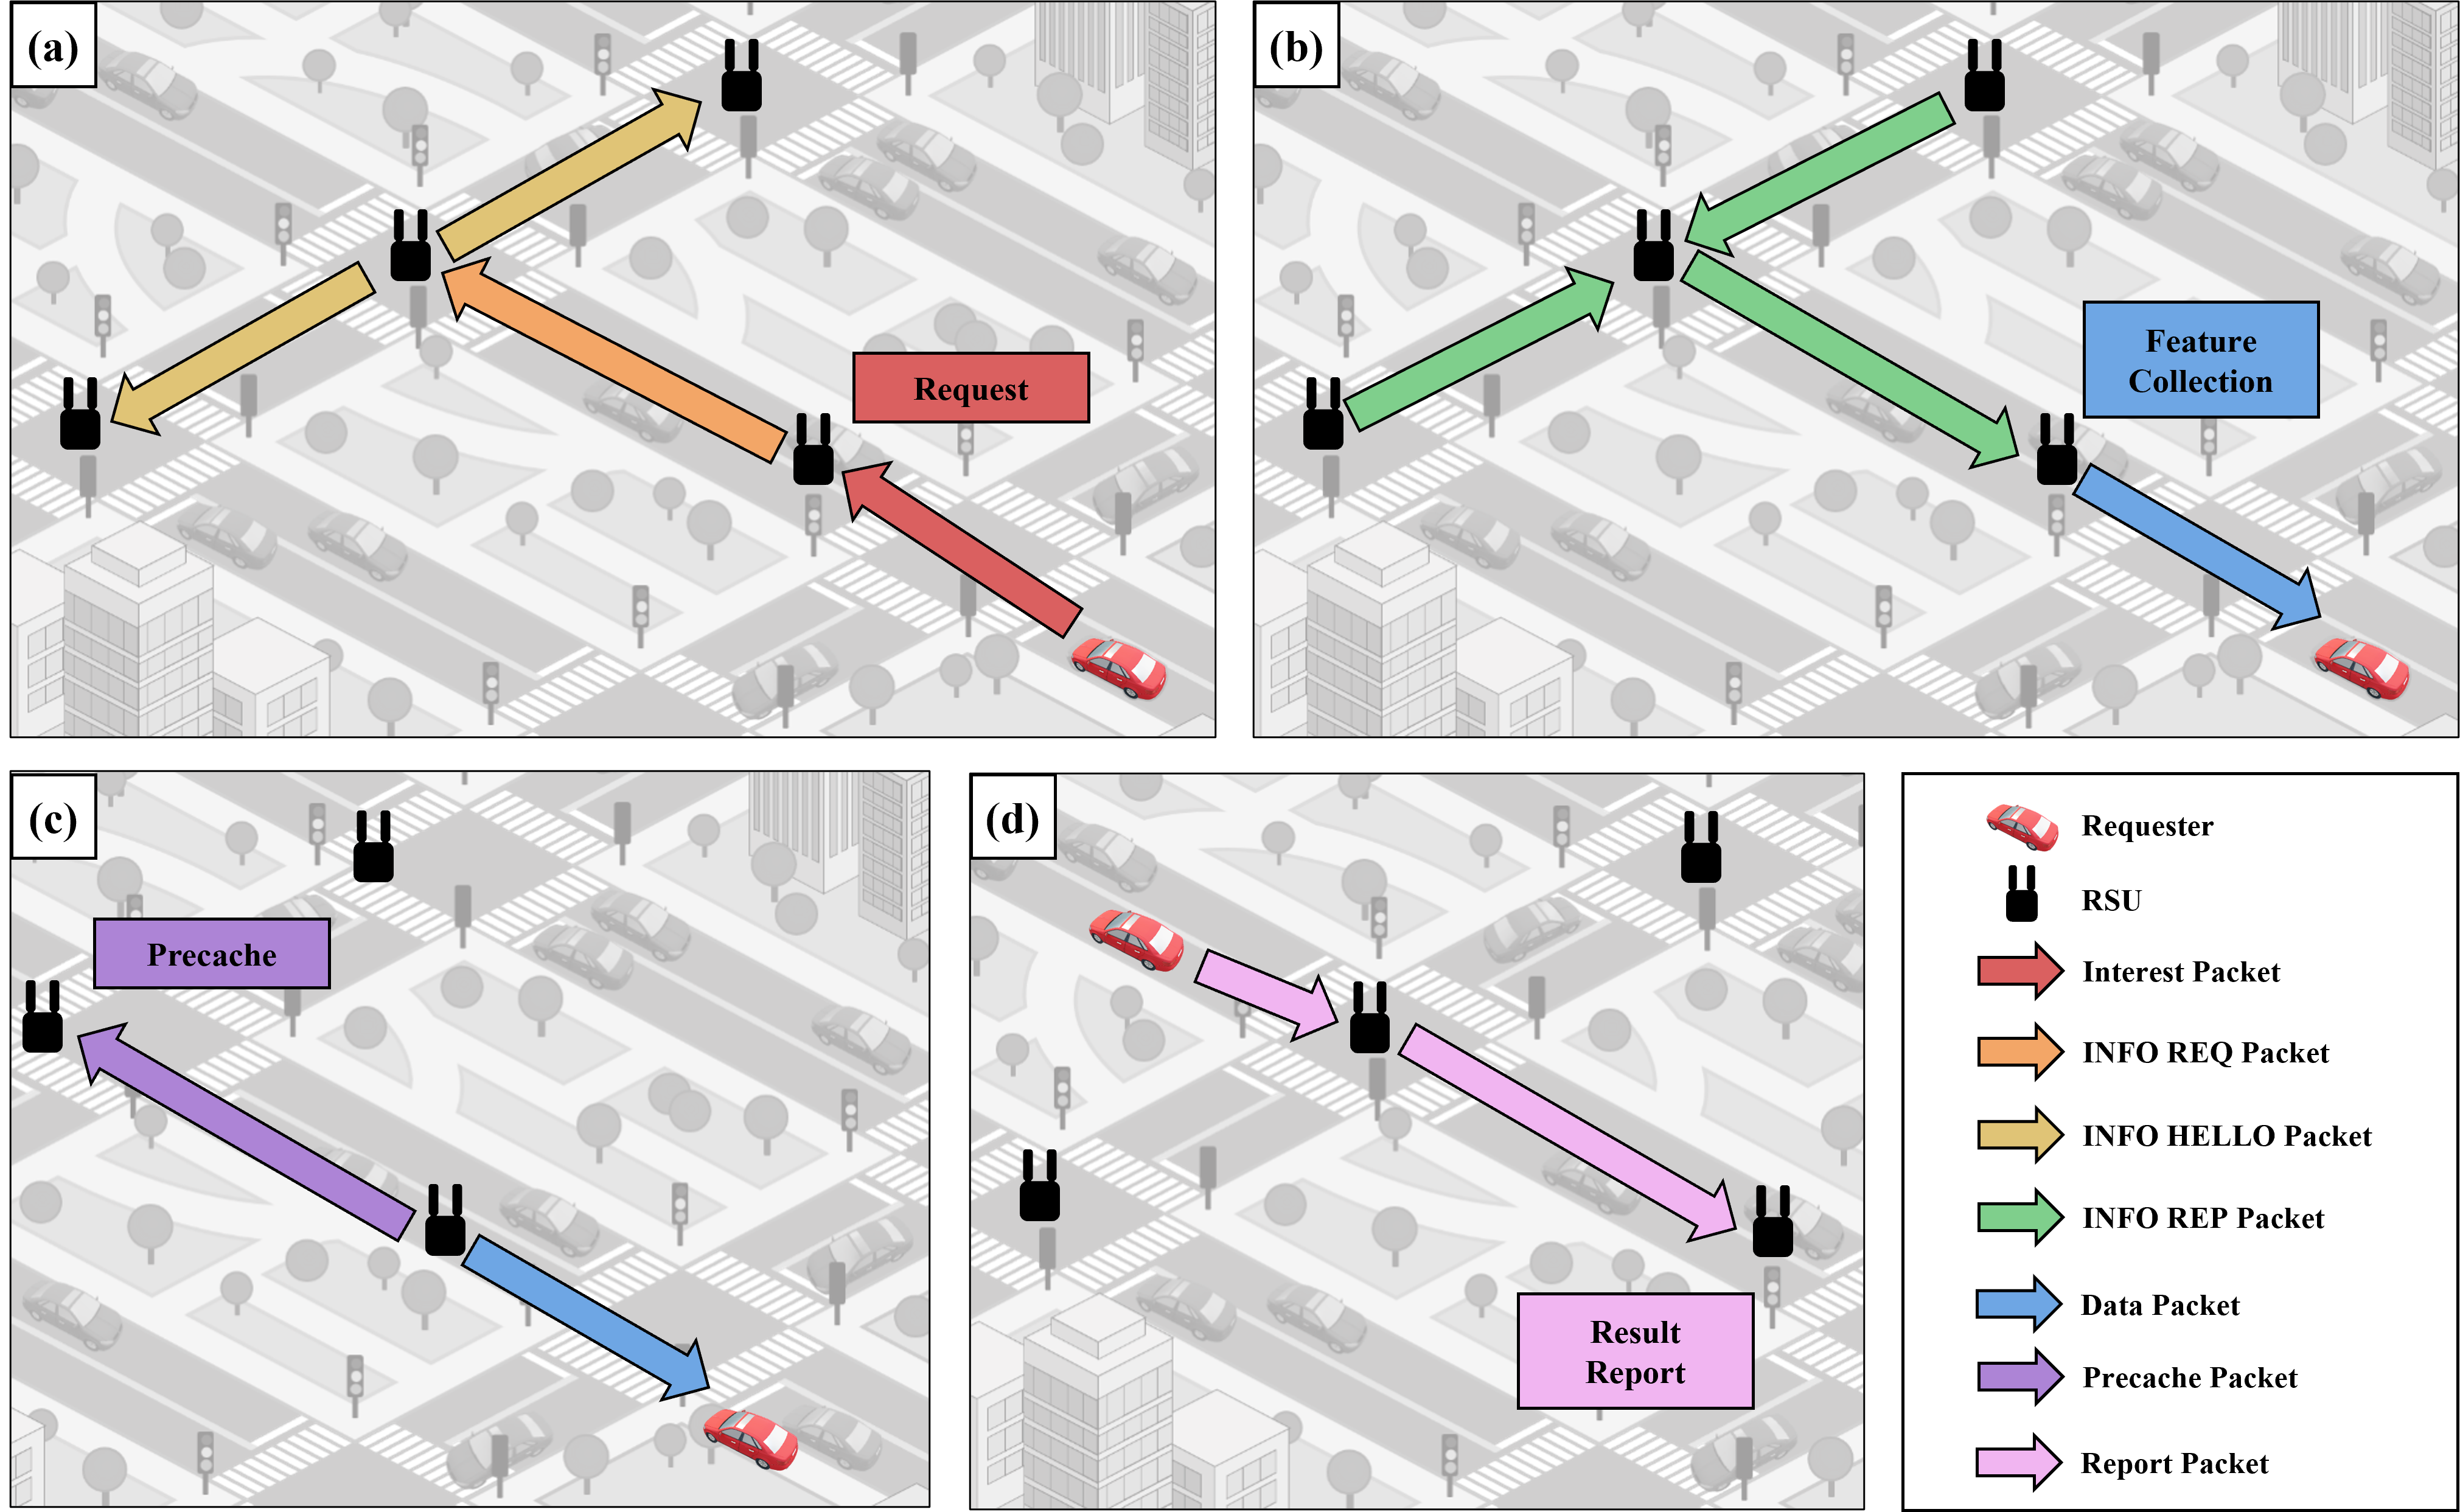
\includegraphics[width=\linewidth]{figure/overview.png}
\caption{Communication scenario overview of the proposed proactive content precaching scheme in CCVNs.}
\label{fig:overview}
\end{figure*}

As illustrated in Fig.~\ref{fig:overview}, the proposed proactive content precaching scheme operates in five main phases.
In Phase 1, the precaching scenario is initiated when a vehicle enters the coverage area and transmits an INTEREST packet containing real-time kinematic metrics to request content.
The current serving RSU processes this request and initializes a Pending Data Table (PDT) to manage local vehicle and traffic states.
In Phase 2, the current RSU exchanges traffic context with adjacent nodes via wired links.
It sends an INFO REQ packet to the subsequent RSU, which then broadcasts an INFO HELLO packet to neighboring RSUs.
Neighboring RSUs reply with merge count data using INFO REP packets, and the next RSU returns a consolidated INFO REP packet to the current RSU.
In Phase 3, the current RSU aggregates the gathered data into a 30-dimensional feature snapshot and inputs it into the H-ST-MBAN to execute dwell-time inference, yielding predictions for the current and next residency times, $\hat{\tau}_{\text{cur}}$ and $\hat{\tau}_{\text{nxt}}$.
In Phase 4, the current RSU computes the deliverable chunk count, $N_{\text{chunk}}$, based on the estimated $\hat{\tau}_{\text{cur}}$ and available bandwidth.
It then forwards a PRECACHE packet containing the next chunk index and $\hat{\tau}_{\text{nxt}}$ to the next RSU, which proactively fetches and caches the required content chunks from the network before the vehicle arrives.
In Phase 5, after the vehicle exits the coverage and records its actual dwell times, it transmits a REPORT packet back to the RSU infrastructure.
This feedback updates the local dataset queue to enable continuous edge fine-tuning through the model swap mechanism.

The collected dwell times are immediately combined with the original input feature vector and added to the local dataset of the RSU. If the RSU lacks a pre-trained model and its local dataset reaches full capacity, it transmits the accumulated information to a centralized learning server. The centralized server receives comprehensive dataset information from all RSUs operating within the region and accumulates a global dataset. Once the global dataset reaches a sufficient volume, the server performs a complete training cycle to learn the spatial characteristics of the traffic environment. The server then distributes the fully trained network parameters to all participating RSUs across the regional grid. RSUs equipped with this pre-trained model subsequently perform local fine-tuning whenever their individual datasets become full. This continuous local adaptation allows the model to reflect the road geometry, traffic signal patterns, and congestion characteristics of each specific intersection.

\section{Proposed Precaching Scheme} \label{sec:architecture}
To realize the key contributions outlined previously, this section describes the proactive content precaching procedure driven by the proposed H-ST-MBAN and its underlying architectural design.
The first subsection explains the mechanism by which a vehicular content request triggers the generation and aggregation of a feature vector.
Subsequently, the second subsection presents the architecture of the H-ST-MBAN model and describes how the model infers the vehicular dwell times.
The third subsection elaborates on the utilization of the predicted dwell times to execute the proactive content precaching operations across the infrastructure nodes.
Finally, the fourth subsection outlines the procedures for collecting ground-truth labels and reporting these metrics, discussing the methodologies applied for the pre-training and periodic local adaptation of the predictive model.

\subsection{Feature Collection via Content Requests} \label{sec.prop.A}
The proactive caching procedure within the proposed framework is initiated when a vehicle issues a content request within the communication range of an RSU.
If the vehicle remains outside the effective communication boundary, it maintains a standby state until physical entry occurs.
Upon entry, the vehicle transmits an INTEREST packet containing its unique vehicle identifier, the target content identifier, the requisite starting chunk index, and real-time kinematic metrics such as position, velocity, inter-vehicle distance, required lane changes, and the subsequent topological route.
The receiving RSU processes this packet and commences content provisioning in accordance with standard Content-Centric Networking (CCN) procedures.
Simultaneously, the RSU initializes a Pending Data Table (PDT) using the vehicle and content identifiers as primary keys, recording the physical state of the requesting vehicle.
The RSU enriches this table by appending locally observable variables including traffic signal states, remaining signal phase duration, the mean speed of vehicles within the coverage area, and the absolute communication radius.
Furthermore, the infrastructure calculates and logs the distance to the intersection center, denoted as $d_{\text{rsu}}$, and the estimated traversal time, denoted as $t_{est}$, based on the reported position and velocity vectors.
To capture directional dynamics, the RSU assigns a binary flag of 1 if the vehicle is departing from the intersection, and 0 if it is approaching.
The infrastructure node also identifies the specific lane occupied by the requesting vehicle to collect granular metrics, including the instantaneous and average speed of the preceding vehicle, the total number of vehicles ahead, and the localized queue length and lane occupancy rate.
Following route extraction, the RSU updates the PDT with the remaining traversal distance within the current coverage zone, the distance to the next RSU entry point, and the distance to the next RSU exit boundary.
By integrating periodic beacon messages, the system computes the real-time average vehicle speed and accounts for vehicles that have not yet exited the coverage zone, ensuring the density metrics reflect current physical conditions.

To acquire complementary spatial states from the subsequent intersection, the current RSU transmits an INFO REQ packet over the wired Infrastructure-to-Infrastructure (I2I) link.
This query packet embeds the originating RSU identifier, the targeted vehicle identifier, and the requested content identifier.
Upon receiving the INFO REQ packet, the subsequent RSU logs the request into its own pending request table.
The subsequent RSU then replaces the source identifier with its own and broadcasts an INFO HELLO packet to its adjacent neighboring infrastructure nodes.
These neighboring nodes evaluate their local average speed management tables to count the number of vehicles anticipated to merge onto the route toward the subsequent RSU, defined as $n_{merge,nxt}$.
The neighbors transmit this aggregated merge count back to the subsequent RSU via an INFO REP packet, alongside the original vehicle and content identifiers.
Concurrently, the subsequent RSU computes its own localized variables, including its current signal state, phase duration, local average speed, downstream queue length, lane occupancy, and the count of preceding vehicles on the anticipated path, denoted as $n_{ahead,nxt}$.
The subsequent RSU synthesizes its internal metrics with the received merge counts and forwards a final consolidated INFO REP packet back to the originating RSU.
Consequently, the initial serving RSU obtains a representation of the downstream conditions, encompassing traffic states, expected vehicular density, and signal timing parameters.

\begin{table}[!t]
  \renewcommand{\arraystretch}{1.1}
  \caption{Input feature enumeration with branch category assignments}
  \label{tab:features}
  \centering
  \begin{tabular}{@{}lp{5.0cm}c@{}}
    \toprule
    \textbf{Symbol} & \textbf{Description} & \textbf{Category} \\
    \midrule
    $r_{\text{cov}}$          & RSU communication coverage radius fixed at 800\,m                            & K \\
    $d_{\text{rsu}}$          & Physical distance between consecutive RSUs                                   & K \\
    $\text{direct}$           & Vehicle direction relative to RSU represented by 0 for approaching and 1 for departing      & K \\
    $d_{l,c}$                 & Remaining distance to current RSU coverage boundary                          & K \\
    $d_{e,n}$                 & Remaining distance to next RSU coverage entry point                          & K \\
    $d_{l,n}$                 & Distance to next RSU coverage exit boundary                                  & K \\
    $v_{c,a}$                 & Mean vehicle speed within current RSU coverage based on historical queue average    & K, S \\
    $v_{n,a}$                 & Mean vehicle speed within next RSU coverage based on historical queue average       & K, S \\
    $\text{tls}_{c}$          & Traffic signal state at current RSU intersection with cyclical encoding       & T \\
    $\text{tls}_{n}$          & Traffic signal state at next RSU intersection with cyclical encoding          & T \\
    $\text{tlt}_{c}$          & Time remaining until next signal phase change at current RSU                 & T \\
    $\text{tlt}_{n}$          & Time remaining until next signal phase change at next RSU                    & T \\
    $n_{t,0}$                 & Vehicle count heading toward next RSU from current RSU coverage zone         & S \\
    $n_{t,1}$                 & Vehicle count heading toward next RSU from neighbor RSU 1 coverage zone      & S \\
    $n_{t,2}$                 & Vehicle count heading toward next RSU from neighbor RSU 2 coverage zone      & S \\
    $n_{t,3}$                 & Vehicle count heading toward next RSU from neighbor RSU 3 coverage zone      & S \\
    $n_{\text{cur}}$          & Total vehicle count within current RSU coverage representing absolute density & S \\
    $n_{\text{nxt}}$          & Total vehicle count within next RSU coverage representing absolute density    & S \\
    $n_{\text{ahead,cur}}$    & Number of vehicles ahead of requesting vehicle on current road edge          & S \\
    $n_{\text{ahead,nxt}}$    & Number of vehicles ahead of requesting vehicle approaching next RSU          & S \\
    $v_{\text{ahead,avg}}$    & Mean speed of vehicles directly ahead on the same edge                       & K, S \\
    $d_{\text{leader}}$       & Gap distance to the immediately preceding leader vehicle                     & K \\
    $v_{\text{leader}}$       & Instantaneous speed of the leader vehicle                                    & K \\
    $q_{\text{len,cur}}$      & Queue length at current RSU intersection measured by halting vehicle count   & T, S \\
    $q_{\text{len,nxt}}$      & Queue length at next RSU intersection measured by halting vehicle count      & T, S \\
    $\text{occ}_{\text{cur}}$ & Real-time lane occupancy rate at current RSU ranging from 0 to 1             & S \\
    $\text{occ}_{\text{nxt}}$ & Real-time lane occupancy rate at next RSU ranging from 0 to 1                & S 	 \\
    $t_{\text{est}}$          & SUMO network-based estimated traversal time for the current road edge        & K, S \\
    $n_{\text{merge,nxt}}$    & Number of competing vehicles merging toward next RSU from adjacent lanes     & S \\
    $\Delta_{\text{lane}}$    & Number of lane changes required to reach next RSU                            & K, S \\
    \bottomrule
  \end{tabular}
\end{table}

The originating RSU merges the received external data with its local PDT entries using the vehicle and content identifiers as relational keys.
To maximize representational efficiency, the integrated data elements are explicitly categorized into three discrete semantic branches prior to computation: kinematic, traffic control, and social variables.
Specifically, the feature domains consist of the Kinematic (K) branch representing vehicle motion and spatial distance parameters, the Traffic Control (T) branch capturing signal phases and timing information, and the Social (S) branch representing surrounding vehicle density and queue metrics.
The resulting feature vector and its corresponding domain categories are structurally defined as presented in Table~\ref{tab:features}.
Because this formulation constructs an instantaneous snapshot utilizing small control packets during ongoing content provision, it reduces the overall communication load compared to continuous time-series trajectory tracking.
The separation between background feature aggregation and active content delivery guarantees that physical service quality remains uncompromised.
This domain-specific categorization empowers the computational framework to extract localized traffic characteristics without relying on a centralized cloud architecture.
By independently resolving contextual metrics at the network edge, the system mitigates the bottleneck phenomena typically observed in centralized processing architectures.

\subsection{Dwell Time Inference and Model Architecture} \label{sec.prop.B}
To determine the volume of proactive chunk prefetching at the subsequent infrastructure node, the active RSU processes the aggregated feature vector from the PDT to infer the current communication residency time ($\hat{\tau}_{\text{cur}}$) and the next residency time ($\hat{\tau}_{\text{nxt}}$).
The system addresses the volatility of V2I environments by proposing the H-ST-MBAN, which is designed to process heterogeneous sensor modalities.
During the initial deployment phase where a pre-trained neural network is unavailable, the RSU uses a fallback mechanism that calculates the durations using basic formulas.
This fallback computes the residency periods by dividing the remaining route distances, derived from the WAVE standard boundaries, by the mean velocity of the surrounding traffic.
The communication framework maintains the PDT and the dataset accumulation queues during this phase to enable data collection for subsequent optimization procedures.

Once the pre-trained H-ST-MBAN model is deployed across the network edges, the infrastructure nodes transition to executing neural inferences.
Unlike visual or sequential structures, vehicular tabular data exhibits differences in scaling properties, encompassing kinematic, spatial, and topological dynamics.
These structural variations induce statistical outliers due to traffic incidents or signal anomalies.
Conventional recurrent architectures or basic multi-layer perceptrons concatenate these heterogeneous arrays, causing the learning process to be dominated by features with larger scales.
Furthermore, this concatenation triggers gradient vanishing or explosion during the periodic local adaptation processes at the computational edges, exacerbating the phenomenon of catastrophic forgetting.


\begin{figure*}[!t]
\centering

\includegraphics[width=\linewidth]{figure/architecture.png}
\caption{Overall architecture of the proposed H-ST-MBAN.}
\label{fig:architecture}
\end{figure*}

To address these structural limitations and improve reliability within the V2I paradigm, the proposed H-ST-MBAN framework is constructed around four computational modules.
The architecture of the proposed H-ST-MBAN is shown in Fig.~\ref{fig:architecture}.
First, the architecture performs Heterogeneous Feature Extraction via Pre-activation Residual Blocks to isolate the different scaling metrics by independently processing the respective categorical domains.
Mathematically, for a given input vector partition $\mathbf{x}_i$, the pre-activation non-linear transformation is defined as follows:
\begin{equation}
\mathbf{z}_i = \mathbf{x}_i + \mathcal{F}(\text{ReLU}(\text{BN}(\mathbf{x}_i)), \mathbf{W}_i)
\end{equation}
where $\text{BN}(\cdot)$ denotes batch normalization, $\mathcal{F}(\cdot)$ represents the residual mapping function, and $\mathbf{W}_i$ represents the learnable weights.
This pre-activation formulation normalizes the domain-specific tensors prior to linear projection, preventing the risk of gradient explosion.
This feature refinement isolates the kinematic, topological, and spatial domains into a unified latent space before feature fusion.

Second, the system incorporates Domain-Level Multi-Head Attention Fusion by processing the independently encoded latent domain vectors as sequential tokens.
Specifically, the individual latent vectors $z_k$, $z_t$, and $z_s$ generated by the first-stage residual blocks are linearly adjusted to possess the identical feature dimension $D_{model}$.
Following this dimensional alignment, these separate vectors are concatenated along the sequence axis to form a unified sequence token matrix $Z = [z_k; z_t; z_s]$.
This structured matrix $Z$ is subsequently provided as the direct input to the multi-head attention layer to initialize the query, key, and value transformations.
Instead of relying on flat tensor concatenations, the proposed framework leverages the scaled dot-product attention paradigm to compute the cross-domain interactions.
The attention output for the query matrices ($\mathbf{Q}$), key matrices ($\mathbf{K}$), and value matrices ($\mathbf{V}$) is mathematically derived through the following expression:
\begin{equation}
\text{Attention}(\mathbf{Q}, \mathbf{K}, \mathbf{V}) = \text{softmax}\left(\frac{\mathbf{Q}\mathbf{K}^T}{\sqrt{d_k}}\right)\mathbf{V}
\end{equation}
where $d_k$ represents the scaling dimension of the latent space.
This attention mechanism computes the interdependence connecting topological traffic signals with queue formations and velocity arrays.
Consequently, the aggregated attention scores produce a contextualized fusion representation that weights the infrastructural constraints affecting vehicular trajectories.

Third, the system implements Robust Deterministic Decoding against Outliers by mapping the attention weighted tensors through a sequence of residual decoders to output deterministic time scalars.
Because the task requires temporal intervals for the content caching schedules, the decoding architecture discards probabilistic distributions to use point-estimate outputs.
To stabilize the backward optimization gradients against traffic anomalies, the model employs the $L_1$ Mean Absolute Error metric defined as:
\begin{equation}
\mathcal{L}_{\text{MAE}} = \frac{1}{N} \sum_{j=1}^{N} \left| y_j - \hat{y}_j \right|
\end{equation}
where $y_j$ and $\hat{y}_j$ denote the ground-truth and inferred temporal residency scalars across the vehicular batches.
This choice of objective function bounds the magnitude of gradient updates caused by statistical outliers inherent in vehicular networks.
Thus, the network parameter optimization converges, regardless of the congestion fluctuations observed within the intersection coverage zones.

Fourth, the framework implements an Adaptive Residual Prior Learning methodology designed to combine non-linear neural processing with the generalization capabilities of GBDTs.
The dwell time inference fuses the dual predictive mechanisms through the adaptive gating equation:
\begin{equation}
\text{Pred}_{\text{final}} = \alpha \times \text{ML\_Pred} + \beta \times \text{NN\_Pred}
\end{equation}
where $\text{ML\_Pred}$ signifies the prior machine learning output and $\text{NN\_Pred}$ represents the neural network estimation.
In this hybrid construct, the scaling coefficients $\alpha$ and $\beta$ serve as learnable parameters updated during local backpropagation cycles at the network edges.
By initializing the network to rely on the decision tree prior, the system establishes an anchor that prevents model collapse.
As the localized infrastructure accumulates traffic patterns, this adaptive gating mechanism scales the neural parameters, shielding the architecture against catastrophic forgetting during periodic local adaptation iterations.

To formally detail the execution of this predictive mechanism, the computational steps of the proposed architecture are summarized in Algorithm~\ref{alg:inference}.
This procedural flow captures the transformation from the raw input snapshots to the final deterministic temporal estimates.
During the execution, the computational load is primarily driven by the multi-head attention and residual decoding operations.
Specifically, the time complexity of the self-attention mechanism scales according to $O(D_{model}^2 \times L)$, where $L$ represents the fixed token sequence length of three.
Because both the sequence length and the model dimension are maintained at bounded values, the overall latency remains strictly constrained.
This mathematically guarantees that the computational load is highly suitable for resource-constrained edge computing environments.

\begin{algorithm}[h]
\caption{H-ST-MBAN Inference Procedure}
\label{alg:inference}
\begin{algorithmic}[1]
\Require Input snapshot $\mathbf{x} = \{\mathbf{x}_k, \mathbf{x}_t, \mathbf{x}_s\}$, Pre-trained weights
\Ensure Dwell time predictions $\hat{\tau}_{\text{cur}}, \hat{\tau}_{\text{nxt}}$
\State Extract $\mathbf{z}_k, \mathbf{z}_t, \mathbf{z}_s$ using independent residual blocks
\State Align dimensions to $D_{model}$ and construct $Z = [z_k; z_t; z_s]$
\State Compute Multi-Head Attention $Z_{attn} = \text{MHA}(Z)$
\State Decode $Z_{attn}$ to obtain neural network prediction $\text{NN\_Pred}$
\State Extract tabular prediction $\text{ML\_Pred}$ using XGBoost prior
\State Compute $\text{Pred}_{\text{final}} = \alpha \times \text{ML\_Pred} + \beta \times \text{NN\_Pred}$
\State \Return $\hat{\tau}_{\text{cur}}, \hat{\tau}_{\text{nxt}}$ from $\text{Pred}_{\text{final}}$
\end{algorithmic}
\end{algorithm}

\subsection{Precaching Procedure Based on Inferred Dwell Time} \label{sec.prop.C}
The calculated dwell-time estimates, $\hat{\tau}_{\text{cur}}$ and $\hat{\tau}_{\text{nxt}}$, serve as the primary foundational variables for scheduling the proactive caching execution.
Based on the inferred value of $\hat{\tau}_{\text{cur}}$, the current serving RSU computes the absolute data volume it can transmit by evaluating the managed average communication bandwidth, denoted as $B_{avg}^{cur}$.
To optimize localized cache storage and circumvent memory fragmentation resulting from variable packet sizing, the architecture mandates a fixed and uniform CCN chunk size, denoted as $S_{chunk}$.
This constant chunk size ensures $O(1)$ algorithmic complexity for memory management while preventing packet segmentation errors caused by lower-layer transmission unit constraints.
When calculating the deliverable chunk count, the system introduces an adaptive safety margin coefficient, denoted as $\eta$, to absorb transient wireless channel fluctuations.
Rather than functioning as a static constant, this coefficient adapts to physical layer conditions via the formulation $\eta(t) = \lambda_1 \cdot \bar{P}_{success}(t) - \lambda_2 \cdot f(\sigma_{channel}^2(t))$, where it processes the recent packet success rate and the measured signal-to-noise ratio variance.
These parameters, specifically $\lambda_1$ and $\lambda_2$, are explicitly defined as independent scaling factors that represent the instantaneous channel state.
This notational choice rigorously avoids any mathematical conflict with the deep learning ensemble parameters utilized within the predictive model.
Consequently, the maximum number of chunks the current infrastructure can transmit is evaluated using the mathematical formula $N_{cur, chunk} = \lfloor \frac{\eta \cdot B_{avg}^{cur} \cdot \hat{\tau}_{\text{cur}}}{S_{chunk}} \rfloor$.

By referencing the initial requested chunk index alongside the calculated $N_{cur, chunk}$ value, the current infrastructure determines the exact terminal chunk number that will complete transmission prior to vehicle departure.
Following this deterministic derivation, the current RSU generates and transmits a specialized PRECACHE packet to the subsequent infrastructure node via the backhaul network.
This strategic communication packet contains the target content identifier, the sequential starting index for the next data block, and the inferred subsequent residency duration $\hat{\tau}_{\text{nxt}}$.
Upon intercepting this packet, the subsequent RSU utilizes the provided $\hat{\tau}_{\text{nxt}}$ value to independently compute its own predictable transmission capacity using the identical algebraic methodology.
The subsequent RSU issues internal INTEREST packets to proactively download the designated sequence of chunks from adjacent routers or the centralized core server in accordance with standard CCN routing protocols.
To mathematically guarantee data freshness and prevent the exhaustion of pending interest tables during vehicle detours, the cached chunks are governed by a Time-To-Live eviction policy.
This proactive expiration mechanism defends the edge storage infrastructure against systemic cache pollution.

\subsection{Vehicle-Measured Dwell Time Ground Truth Reporting} \label{sec.prop.D}
To guarantee the continuous optimization of the localized predictive models, the edge network mandates an operational feedback loop originating from the mobile clients.
As the vehicle crosses the exit boundary of the current RSU, its onboard computing unit locally records the associated infrastructure identifier and the physically measured empirical residency time.
Following standard network protocol, the vehicle periodically broadcasts INTEREST packets to attempt continuous content retrieval from the infrastructure.
Upon physically entering the communication range of the subsequent intersection, the vehicle transmits these INTEREST packets to the new RSU, triggering a distinct and independent content provision process.
This parallel operation initiates the feature collection sequence anew at the subsequent intersection independently of the prior data session.
Simultaneously, the vehicular system activates an internal timer to measure the actual $\tau_{\text{nxt}}$ duration while receiving the prefetched data chunks.
Any segments that were not proactively cached due to estimation variance are requested and retrieved from neighboring nodes utilizing standard name-based resolution mechanisms.

As the vehicle prepares to depart from the coverage zone of this subsequent RSU, it finalizes the aggregation of the true $\tau_{\text{nxt}}$ duration.
The onboard unit encapsulates the vehicle identifier, the target content identifier, the previously stored RSU identifier, and the two verified empirical dwell times into a dedicated REPORT packet.
The vehicle transmits this operational feedback packet to the currently associated infrastructure node over the active wireless interface.
Upon packet reception, the active RSU evaluates the embedded infrastructure identifier; if the identifier does not match its own, the RSU routes the packet backward through the wired topology.
When the originally serving RSU receives the forwarded REPORT packet, it scans its internal PDT to match the relational keys associated with the original vehicle and content identifiers.
The infrastructure node extracts the correlated input feature vector and combines it with the empirical time durations to generate a ground truth record.
This annotated data structure is accumulated into the dedicated local dataset queue to facilitate subsequent supervised machine learning processes.

\subsection{Dataset Training and Two-Track Model Operation} \label{sec.prop.E}
The continuous aggregation of ground truth pairs governs the localized model adaptation under a two-track operation protocol designed to ensure zero service interruption. During the initial deployment phase, the active RSUs lack pre-trained parameters and accumulate empirical data into their local queues. Once a sufficient volume of data accumulates, the infrastructure transmits these dense batches to a centralized cloud server to execute global pre-training. Following mathematical convergence, the central server distributes the identical optimized weights back to every participating RSU. Upon receiving these initialized parameters, the edge nodes transition into an autonomous operational state, eliminating continuous uplink training bottlenecks while adapting to specific intersection anomalies.

To execute this continuous local adaptation without introducing latency into active caching decisions, each RSU natively operates two independent model instances following a distinct ping-pong logic. The content provisioning and dwell-time inference exclusively rely on the active inference model, utilizing the most recently optimized weights to process incoming client requests. Simultaneously, the background standby model monitors the localized dataset queue and executes fine-tuning only after the queue reaches its designated capacity. When the background model successfully finalizes its localized gradient descent updates, the RSU executes a role exchange to promote the updated model. The outdated inference model concludes its final ongoing predictive calculations before being structurally demoted to the standby role, clearing the processed queue for the subsequent optimization cycle.


\section{Performance Evaluations} \label{sec:experiments}

\subsection{Experimental Setup}
To validate the proposed H-ST-MBAN architecture, we construct a microscopic traffic environment utilizing the SUMO framework. The CCVN environment is modeled around complex multi-lane intersection topologies, utilizing the urban road network layouts to capture realistic vehicle trajectories. Within this simulation, vehicles are governed by advanced car-following and lane-changing models that replicate real-world human driving behaviors, including acceleration, deceleration, and lane-merging dynamics. The intersection traffic signals operate on fixed periodic cycles, with a total duration of 90 seconds, comprising 42 seconds of green, 3 seconds of yellow, and 45 seconds of red, and individual phase transitions $T_\text{phase}$ occurring every 30 seconds. To emulate a wide spectrum of congestion states, the simulations inject vehicles at varying generation rates, resulting in traffic densities that span continuously from sparse conditions at 5 veh/km/lane to congested scenarios reaching 25 veh/km/lane.

The networking layer of the simulation implements specific communication parameters to govern the V2I interactions. Each RSU is positioned at the geometric center of major intersections and provides a fixed omnidirectional communication coverage radius of 800 meters, which adheres to the WAVE standard. Consecutive RSUs are deployed at an inter-RSU spacing of 2,400 meters, intentionally creating an 800-meter shadow region between adjacent coverage zones where no V2I signal is available. This topology forces the proactive caching scheduler to time its content delivery before the vehicle enters the dead zone. The V2I links are modeled with standard vehicular networking bandwidth constraints, where packet delivery success rates and channel signal-to-noise ratios fluctuate based on instantaneous vehicle density and physical distance to the RSU antenna. These communication parameters ensure that the predictive models are evaluated under realistic bandwidth constraints and edge-caching deadlines.

To execute the computational aspects of the framework, we utilize a heterogeneous hardware environment that separates global pre-training from local fine-tuning. The initial global pre-training phase is conducted on a high-performance centralized workstation equipped with an Intel Core i9-10900X CPU, 128 GB of DDR4 RAM, and four NVIDIA GeForce RTX 3090 GPUs. This massive computational capacity allows the core server to rapidly process the aggregated global dataset and establish the initial prior weights for the neural network. Conversely, the local fine-tuning phase is simulated under the strict resource constraints typical of standard RSU edge hardware. The edge nodes operate with limited thermal and electrical budgets, restricting peak memory consumption to under 50 MB and requiring fast execution times to prevent inference bottlenecks. This dual-tier hardware configuration accurately reflects the practical deployment constraints of modern intelligent transportation systems.

The underlying dataset comprises over 1,000,000 independent snapshot samples collected systematically across various target intersections. Each snapshot encapsulates a 30-dimensional feature vector containing kinematic, traffic control, and social density variables captured at the exact moment a content request is issued. To ensure model evaluation and prevent temporal data leakage, the dataset is partitioned using a chronological split strategy. Specifically, the dataset is partitioned using a 70:15:15 (Train:Val:Test) ratio, where 70\% of the earliest temporal data is allocated for training, 15\% for validation, and the final 15\% is reserved for testing. This split is reasonable because the deep learning baseline models, including ResNet and LSTM, require a dedicated validation set to tune hyperparameters and execute early stopping, which prevents model overfitting under constrained edge resources. Standard scaling is applied exclusively using the statistics derived from the training set to prevent any forward-looking bias during the validation and testing phases.

\subsection{Baseline Models}
To evaluate the predictive performance of H-ST-MBAN, we benchmark against twelve representative baseline models spanning traditional machine learning, deep learning, and advanced deep tabular paradigms. These include linear and tree-based models such as Logistic Regression (LR) \cite{cox1958}, Random Forest (RF) \cite{breiman2001}, XGBoost \cite{chen2016}, CatBoost \cite{prokhorenkova2018}, and NGBoost \cite{duan2020}. We also evaluate standard deep neural networks including Multi-Layer Perceptron (MLP) \cite{rumelhart1986}, ResNet \cite{he2016}, LSTM \cite{hochreiter1997}, and Gated Recurrent Unit (GRU) \cite{cho2014}. Furthermore, we compare with recent tabular deep learning models, specifically Feature Tokenizer Transformer (FTT) \cite{gorishniy2021}, TabR \cite{gorishniy2024}, and TabPFN \cite{hollmann2023}. These diverse baselines establish a comprehensive evaluation framework to assess the deterministic regression capabilities of our proposed architecture.

\subsection{Learning Curves}
We structure our evaluation through a logical sequence of seven distinct graphs, analyzing model convergence, component contributions, prediction accuracy, edge deployment feasibility, and downstream proactive caching performance.
To evaluate training convergence, we benchmark H-ST-MBAN against twelve representative models, including linear and tree-based ensembles, traditional time-series models, standard deep learning baselines, and advanced deep tabular models.
Figure~\ref{fig:G1} presents the learning curves for the evaluated predictive architectures.
For a transparent comparison, it is critical to state that the X-axis for the machine learning models represents the number of trees, defined as Boosting Rounds.
In contrast, the X-axis for the deep neural networks represents the number of backpropagation updates, explicitly defined as Epochs.
Although these iteration metrics are fundamentally different in their computational mechanics, they are scaled and visually aligned to evaluate the overall optimization trajectory.
Consequently, the analysis strongly focuses on the common goal of both paradigms, which is to achieve convergence stability as the number of iterations progresses.
The resulting curves demonstrate that H-ST-MBAN converges more smoothly and achieves a lower loss compared to the baseline approaches.

\begin{figure}[!t]
\centering
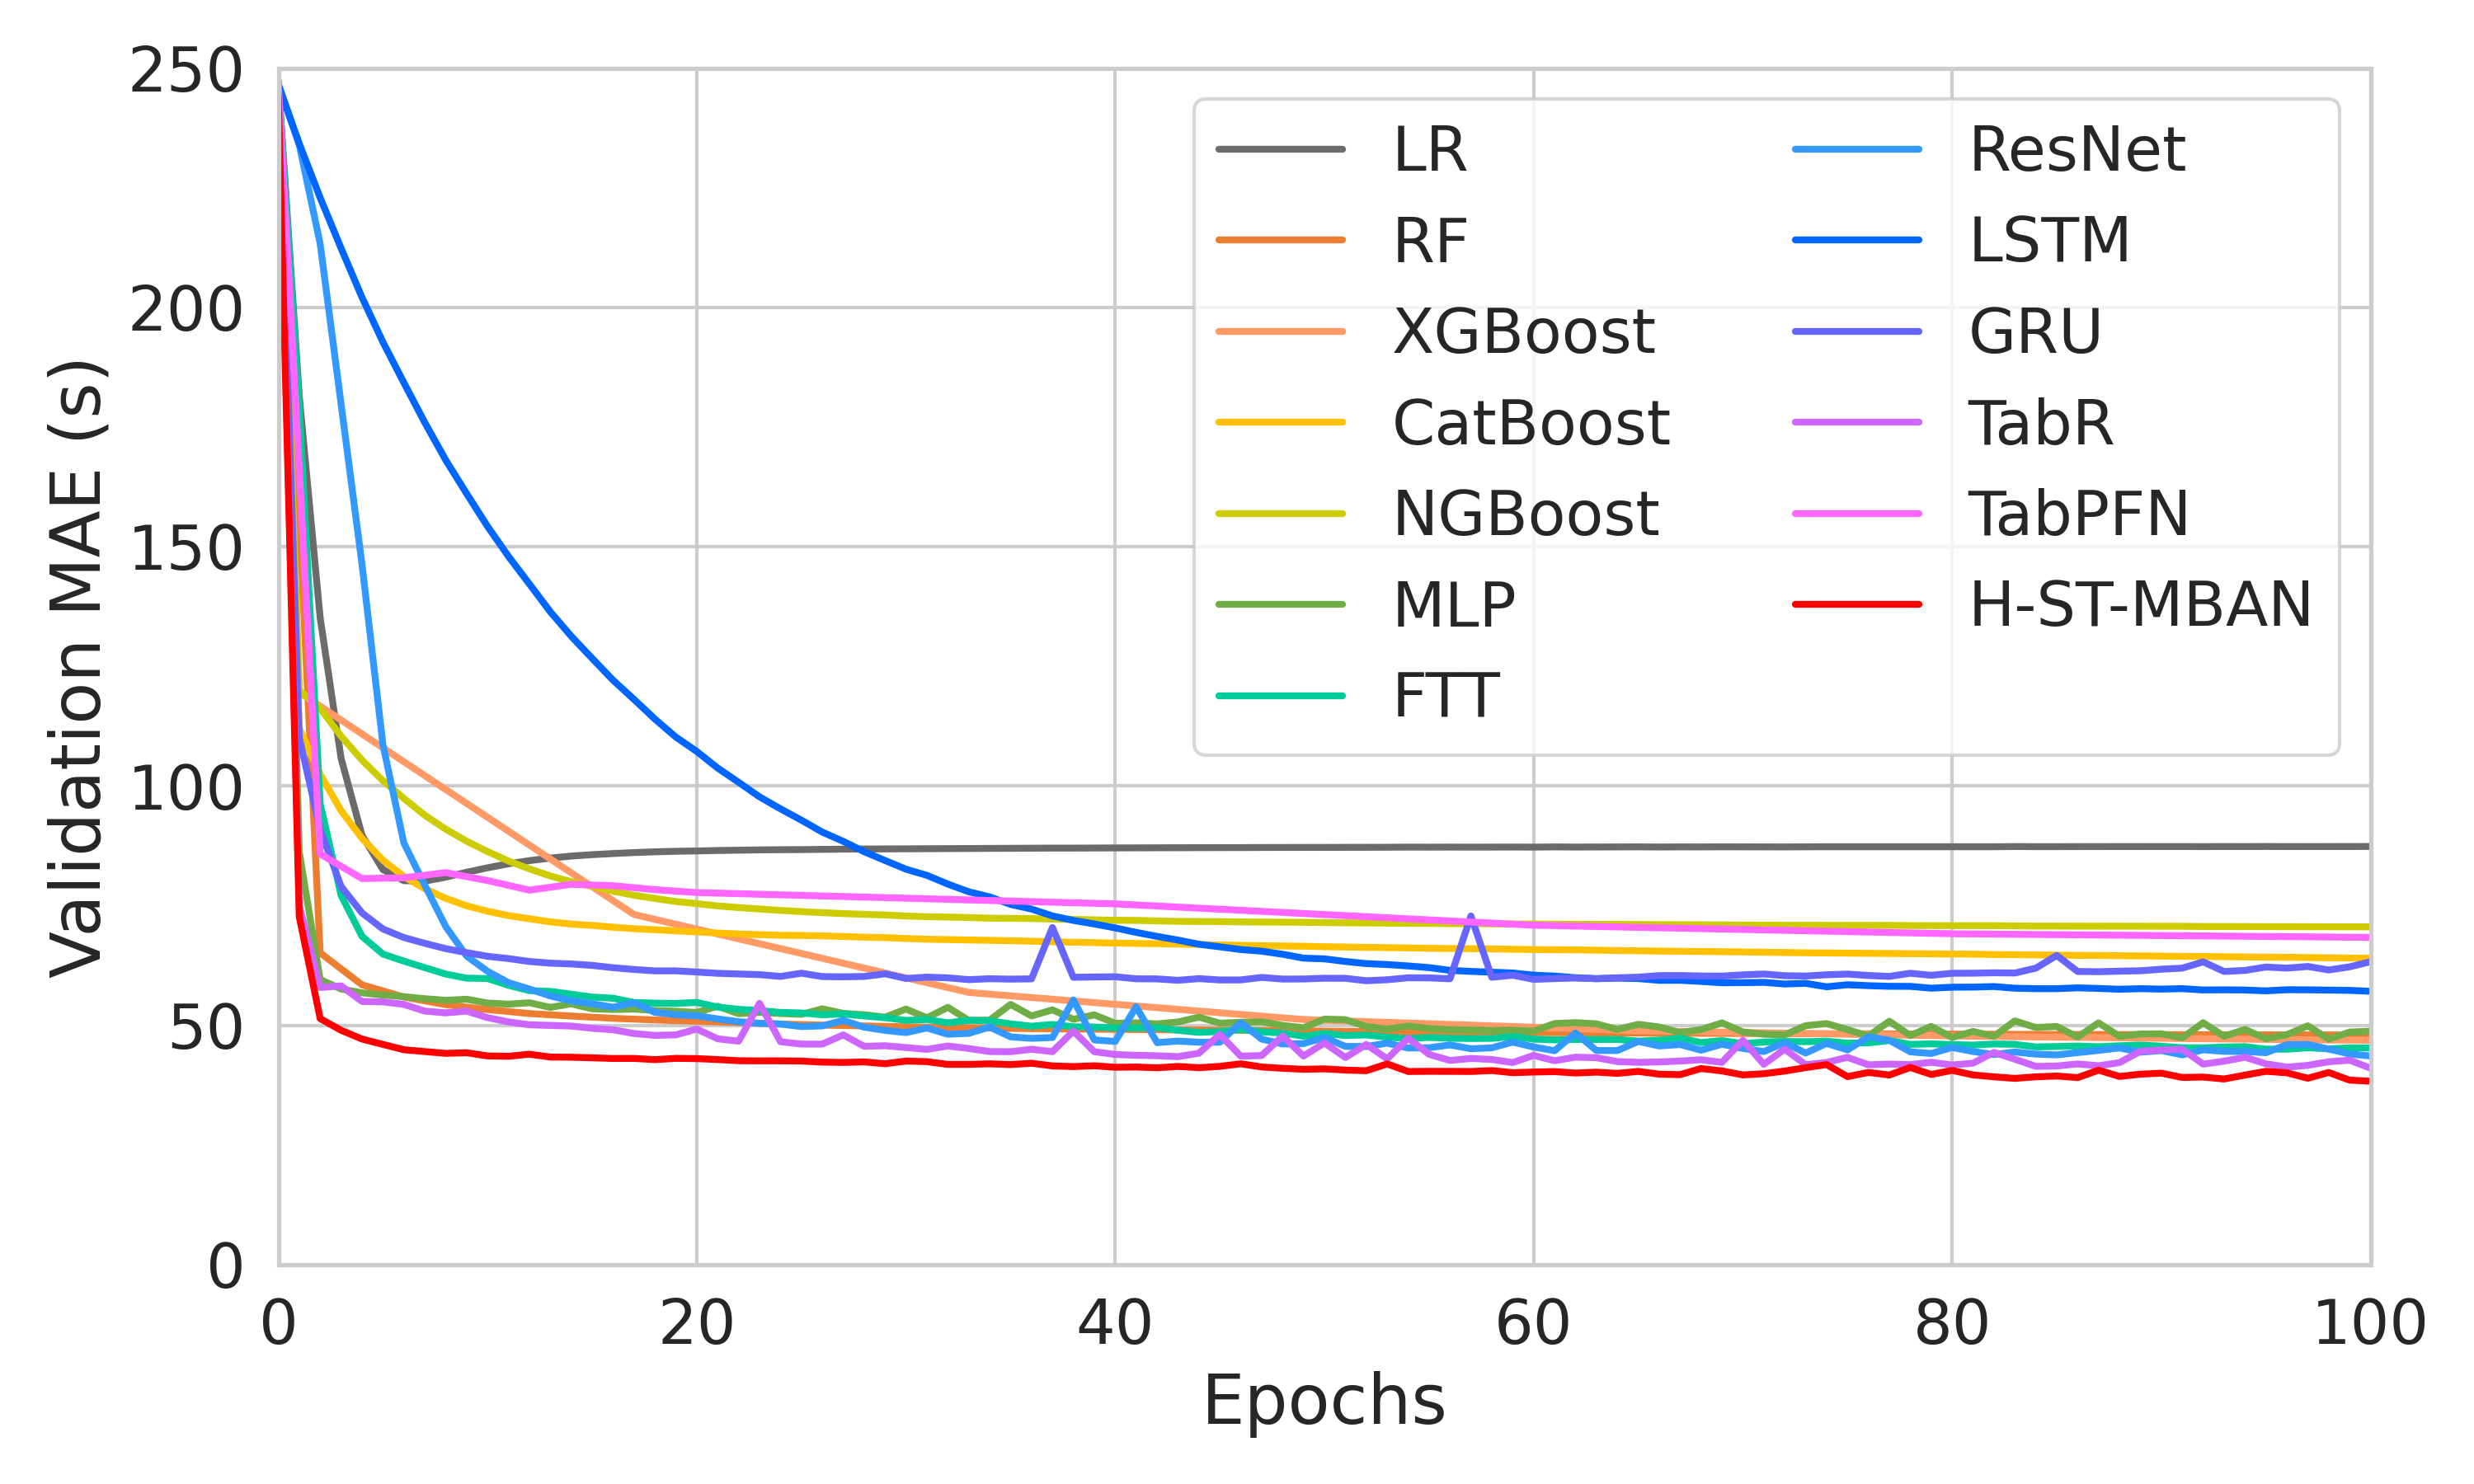
\includegraphics[width=\columnwidth]{figure/G1_learning_curves.png}
\caption{Convergence of H-ST-MBAN compared to baseline models. ML model iterations are aligned with DL epochs for a fair comparison.}
\label{fig:G1}
\end{figure}

\subsection{Ablation Study}
To evaluate the contribution of the heterogeneous multi-branch structure, we conducted an ablation study by modifying the H-ST-MBAN components.
As illustrated in Figure~\ref{fig:G2}, we evaluate three degraded variants to isolate the individual contribution of each architectural feature. The \textit{w/o Attn} variant replaces the MHA mechanism with simple concatenation. The \textit{w/o XGB} variant relies solely on the neural network stream by omitting the GBDT prior. The \textit{Early Fusion} variant concatenates features before encoding instead of using the independent branch structure. The results show that the \textit{w/o XGB} variant suffers a significant performance drop, confirming the necessity of integrating the tabular prior to handle decision boundaries that the neural network struggles to learn alone. The \textit{Early Fusion} variant also exhibits higher error, indicating that the heterogeneous nature of vehicular data benefits from semantic branching to prevent gradient conflicts during encoding. Finally, removing the attention layer in \textit{w/o Attn} degrades convergence and increases error, showing that MHA routes the relevant bottleneck features depending on the specific intersection context. The full H-ST-MBAN model achieves the lowest error and fastest convergence. This collective behavior confirms the powerful synergy between gradient-boosted tabular priors and neural representation learning, where the GBDT stream establishes baseline decisions and the multi-branch neural network stream refines spatio-temporal details.

\begin{figure}[!t]
\centering

\includegraphics[width=\columnwidth]{figure/G2_ablation_study.png}
\caption{Performance of H-ST-MBAN compared to w/o Attn, w/o XGB, and Early Fusion variants.}
\label{fig:G2}
\end{figure}

\subsection{Prediction Accuracy}
Table~\ref{tab:accuracy} summarizes the global prediction performance, evaluated using MAE, Root Mean Square Error (RMSE), and Mean Absolute Percentage Error (MAPE).
H-ST-MBAN yields an MAE of 44.32~s, improving upon the second-best baseline, ResNet, which yields an MAE of 47.10~s. Traditional sequential models, namely LSTM and GRU, show higher error, exhibiting higher MAEs of 96.90~s and 101.75~s, respectively, which may be attributed to the difficulty of inferring temporal dynamics from a single event-driven snapshot.
The reduction in MAE achieved by H-ST-MBAN compared to ResNet is primarily due to the incorporation of the gradient boosting tabular prior stream, which models sharp decision boundaries.
In contrast, pure deep neural network structures struggle to learn these non-linear tabular divisions from unstructured variables.
Additionally, the multi-branch self-attention fusion allows H-ST-MBAN to weight dynamic spatial and temporal components based on signal timings, which mitigates regression error.

Figure~\ref{fig:G3} visualizes the True vs. Predicted dwell times for both current and next targets.
In these plots, H-ST-MBAN demonstrates tighter clustering along the identity line, indicating stability against outliers that typically disrupt V2I schedules.
The prediction for the next RSU dwell time, $\hat{\tau}_{\text{nxt}}$, shows slightly more variance and error than the current RSU dwell time, $\hat{\tau}_{\text{cur}}$. This variance is physically intuitive because downstream traffic conditions at the next intersection are subject to additional random perturbations during the inter-RSU traversal interval. Despite this inherent uncertainty, the proposed design maintains a tight error boundary, confirming the benefit of incorporating multi-intersection social features.
This occurs because predicting further into the future involves a more complex spatial-temporal space, particularly since the vehicle can branch into one of four possible next RSUs at the upcoming intersection.
To address this spatial-temporal uncertainty, the caching scheduler can implement a dynamic correction factor that adjusts prefetching thresholds based on branching probabilities.
This compensation mechanism mitigates the impact of estimation variance on subsequent roadside edge cache hit rates.

\begin{table}[!t]
\centering
\caption{Global Prediction Accuracy Across 13 Models. H-ST-MBAN achieves the lowest MAE and RMSE.}
\label{tab:accuracy}
\begin{tabular}{lcccc}
\toprule
\textbf{Model} & \textbf{MAE (s) $\downarrow$} & \textbf{RMSE (s) $\downarrow$} & \textbf{MAPE (\%) $\downarrow$} & \textbf{$R^2$ $\uparrow$} \\
\midrule
\textbf{H-ST-MBAN} & \textbf{44.32} & \textbf{90.54} & \textbf{17.90} & \textbf{0.8618} \\
ResNet & 47.10 & 92.27 & 23.16 & 0.8565 \\
TabPFN & 66.62 & 152.33 & 21.30 & 0.6089 \\
TabR & 80.59 & 170.40 & 27.32 & 0.5106 \\
XGB & 81.95 & 181.94 & 23.88 & 0.4420 \\
CatBoost & 83.02 & 187.83 & 24.72 & 0.4053 \\
RF & 83.75 & 185.30 & 26.59 & 0.4212 \\
LSTM & 96.90 & 196.65 & 32.44 & 0.3481 \\
LR & 97.42 & 199.67 & 49.57 & 0.3280 \\
GRU & 101.75 & 201.36 & 40.40 & 0.3165 \\
FTT & 103.52 & 194.94 & 39.61 & 0.3594 \\
MLP & 108.02 & 212.61 & 35.89 & 0.2380 \\
NGBoost & 109.18 & 199.09 & 76.12 & 0.3318 \\
\bottomrule
\end{tabular}
\end{table}

\begin{figure}[!t]
\centering

\includegraphics[width=0.48\columnwidth]{figure/G3-1_pred_vs_true_cur.png}
\hfill

\includegraphics[width=0.48\columnwidth]{figure/G3-2_pred_vs_true_nxt.png}
\caption{Scatter plots of True vs. Predicted Dwell Time for current target ($\hat{\tau}_{\text{cur}}$, left) and next target ($\hat{\tau}_{\text{nxt}}$, right).}
\label{fig:G3}
\end{figure}

\begin{table}[!t]
\centering
\caption{Fine-Tuning Complexity and RSU Edge Feasibility (1 Round, Q=5000)}
\label{tab:complexity}
\begin{tabular}{@{}lc@{}}
\toprule
\textbf{Metric} & \textbf{H-ST-MBAN} \\
\midrule
Parameters (M) & 1.385 \\
Model Size (MB) & 5.32 \\
Training Time (s) & 1.93 \\
Peak Memory (MB) & 47.69 \\
FLOPs (M) & 198,750 \\
\bottomrule
\end{tabular}
\end{table}

\subsection{Optimal Queue Size Analysis}
The global pre-training phase is executed on a high-performance workstation equipped with an Intel Core i9-10900X CPU, 128 GB of RAM, and four NVIDIA GeForce RTX 3090 GPUs, while the local fine-tuning phase must be viable on resource-constrained RSU edge hardware.
To evaluate edge feasibility, we analyze the computational complexity of the model and its memory footprint.
In dynamic vehicular environments, edge computing boards operate under strict thermal and electrical constraints, which limits the deployment of oversized deep learning parameters.
Moreover, because dwell-time prediction must be completed within milliseconds of a request packet arrival, memory access latency must be minimized to avoid buffering bottlenecks.
These edge constraints necessitate lightweight models that do not exceed local computing bounds while maintaining accuracy.
Specifically, as detailed in Table~\ref{tab:complexity}, the empirical measurements of the proposed H-ST-MBAN architecture exhibit optimized computational complexity tailored for edge deployment.
Considering the general hardware computing specifications of contemporary roadside units, which typically feature low-power embedded processors and constrained RAM capacities, the model maintains a storage footprint of 5.32~MB.
Furthermore, the total parameter count is restricted to 1.385 million, ensuring that the learnable weights are retained within the local memory cache without triggering excessive paging.
During the localized adaptation phase, the peak memory utilization is contained at 47.69~MB, and the fine-tuning execution is completed in 1.93 seconds per update cycle.
These physical characteristics allow the proposed model to operate on standard RSU hardware without imposing detrimental computational overhead or inducing thermal bottlenecks.
Consequently, the predictive framework executes both instantaneous dwell-time inference and periodic local fine-tuning without disrupting the primary communication and caching operations of the edge router.

As shown in Figure~\ref{fig:G4-1} and Figure~\ref{fig:G4-2}, we analyze the trade-off between the fine-tuning queue size and local prediction stability. A queue size of 5000 is chosen as the optimal operating parameter based on three analytical justifications. First, this value represents the knee of the curve regarding cost-effectiveness, where the marginal gain in stability, which represents a variance reduction, drops when scaling past 5000. Second, to ensure statistical confidence, the MAE standard deviation, represented by SEM, is below 1.0, yielding approximately 0.29~s, at $Q=5000$, preventing erratic model updates. Third, this configuration provides an adequate ITS SLA margin. According to ITS recommended standards, caching and model updates should occur every 15--60 minutes \cite{office2021}. Accumulating a queue of 5000 snapshots takes approximately 43 minutes, placing the update frequency in the middle of this 15--60 minutes ITS standard interval and providing a safety buffer against varying traffic density.

\begin{figure}[!t]
\centering
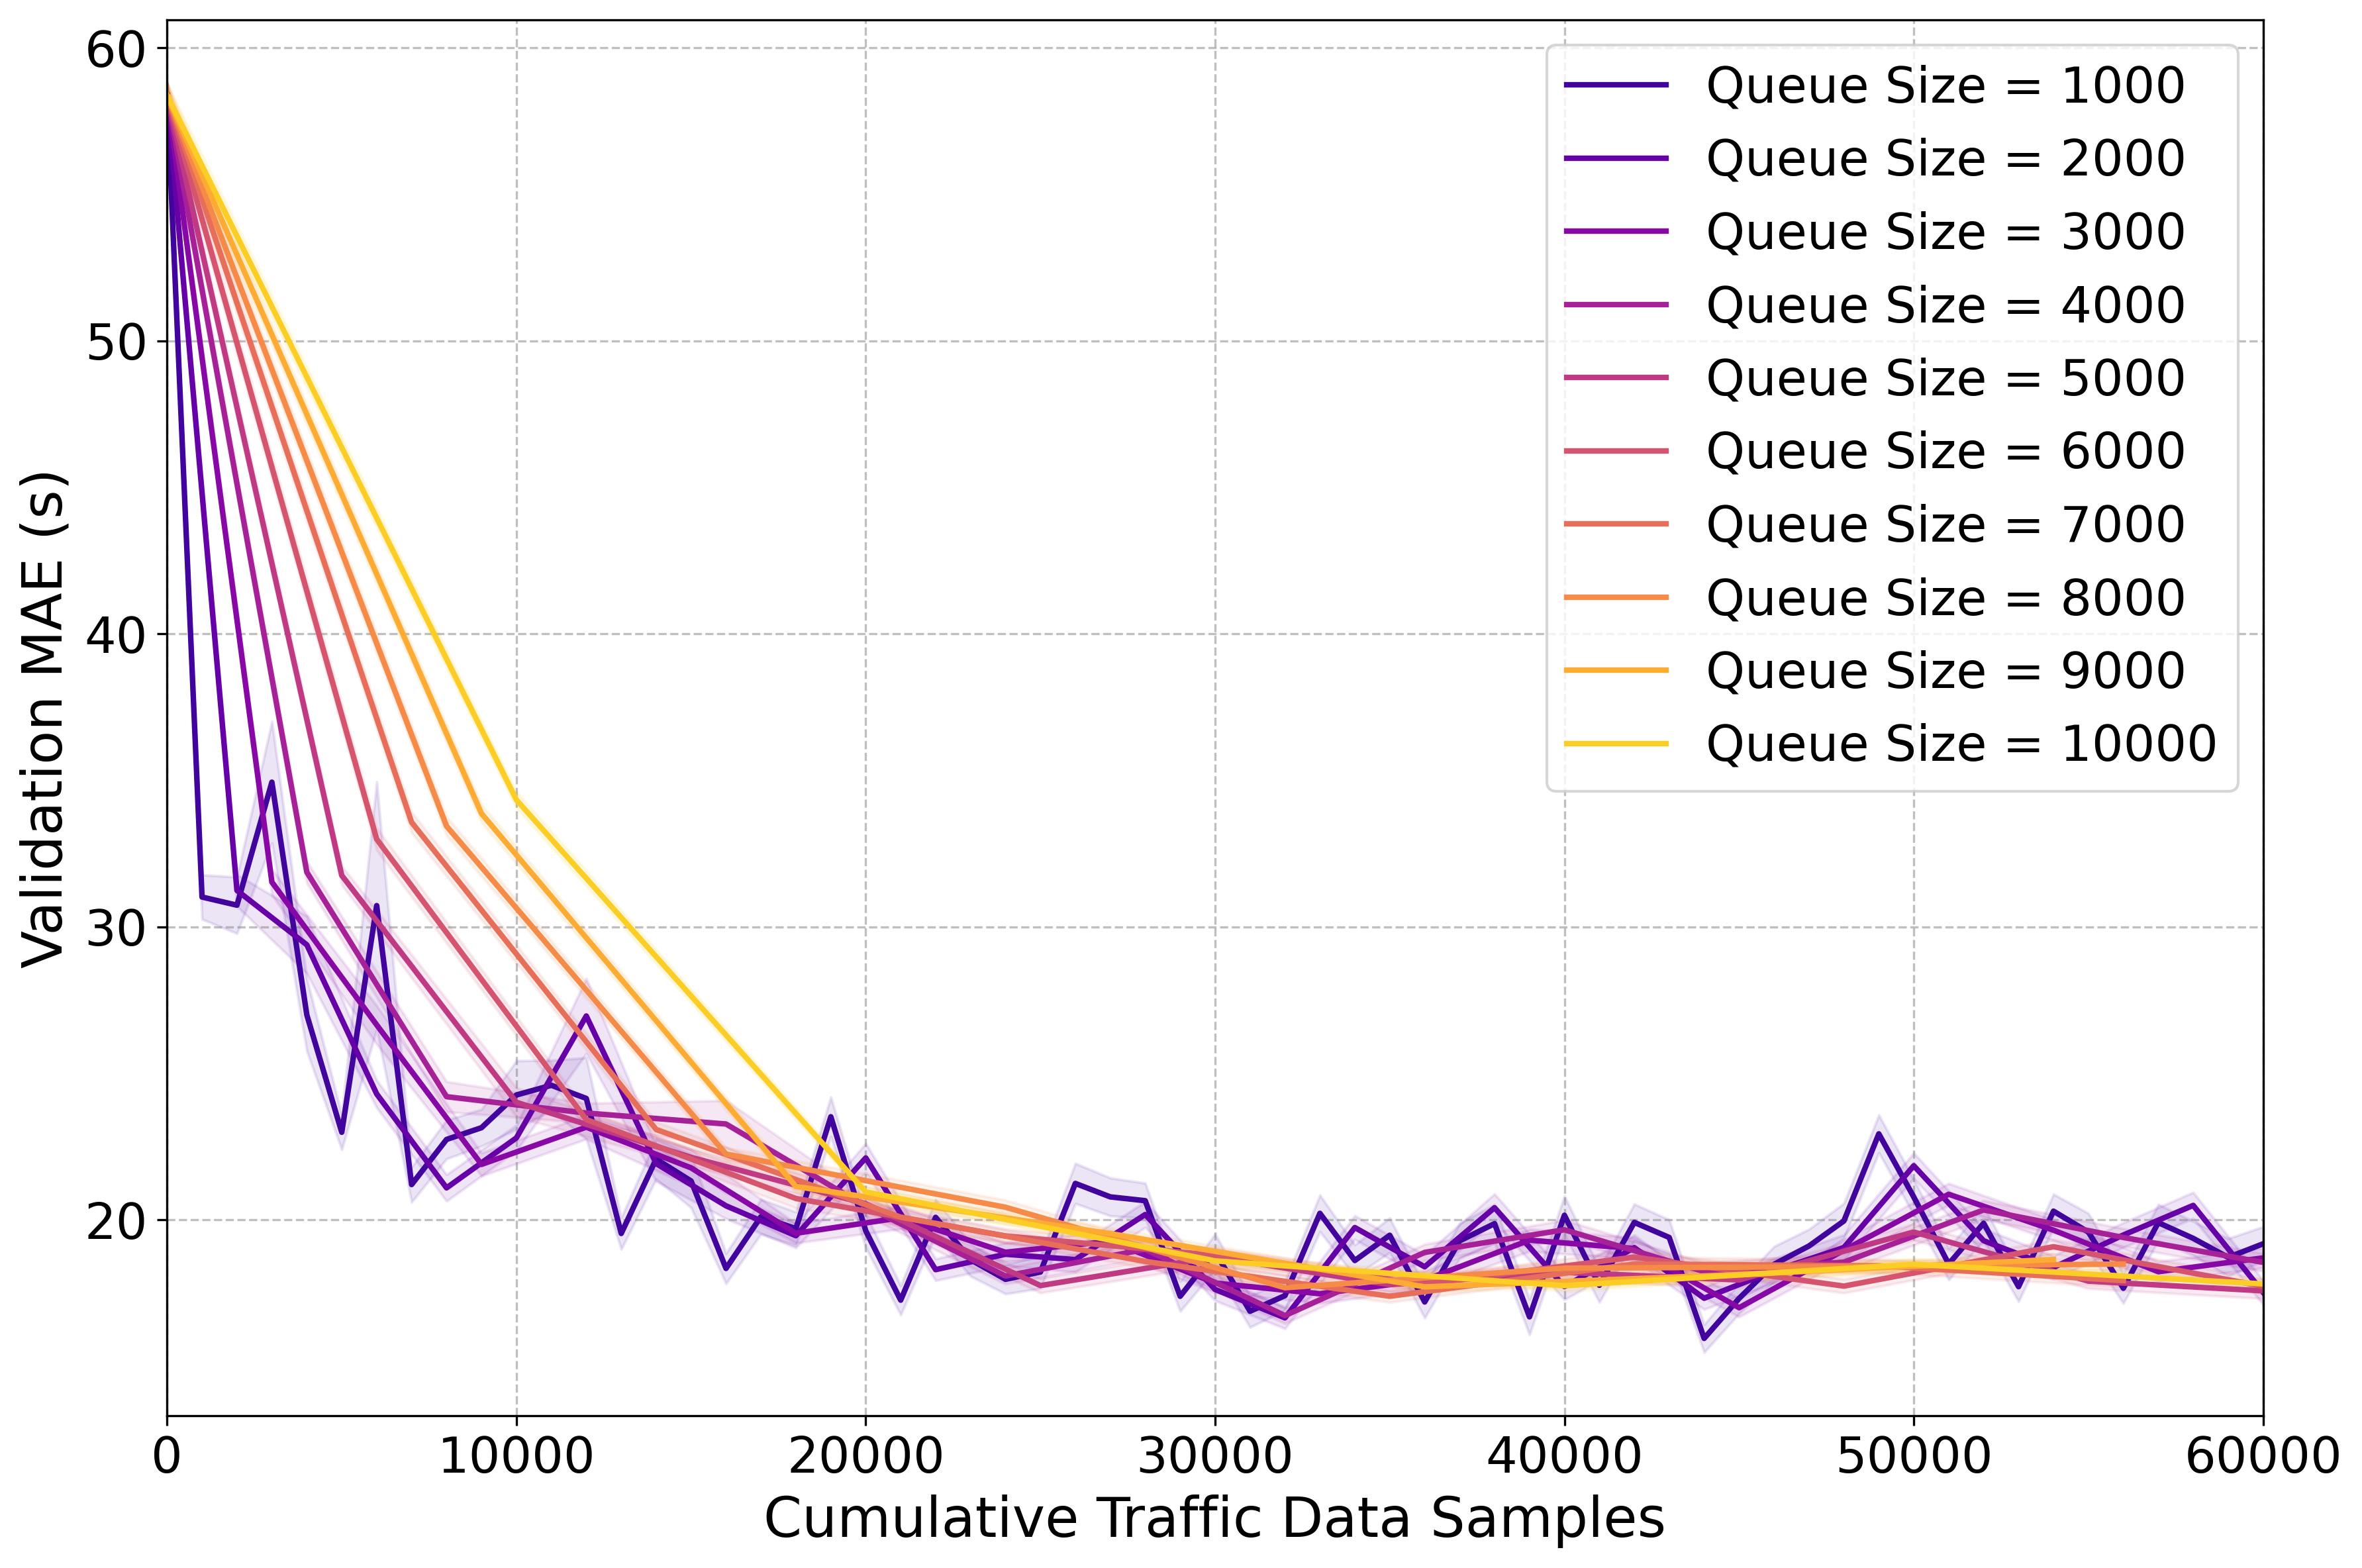
\includegraphics[width=\columnwidth]{figure/G4-1_cumulative_mae_validation.png}
\caption{H-ST-MBAN cumulative validation MAE curves by queue size.}
\label{fig:G4-1}
\end{figure}

\begin{figure}[!t]
\centering
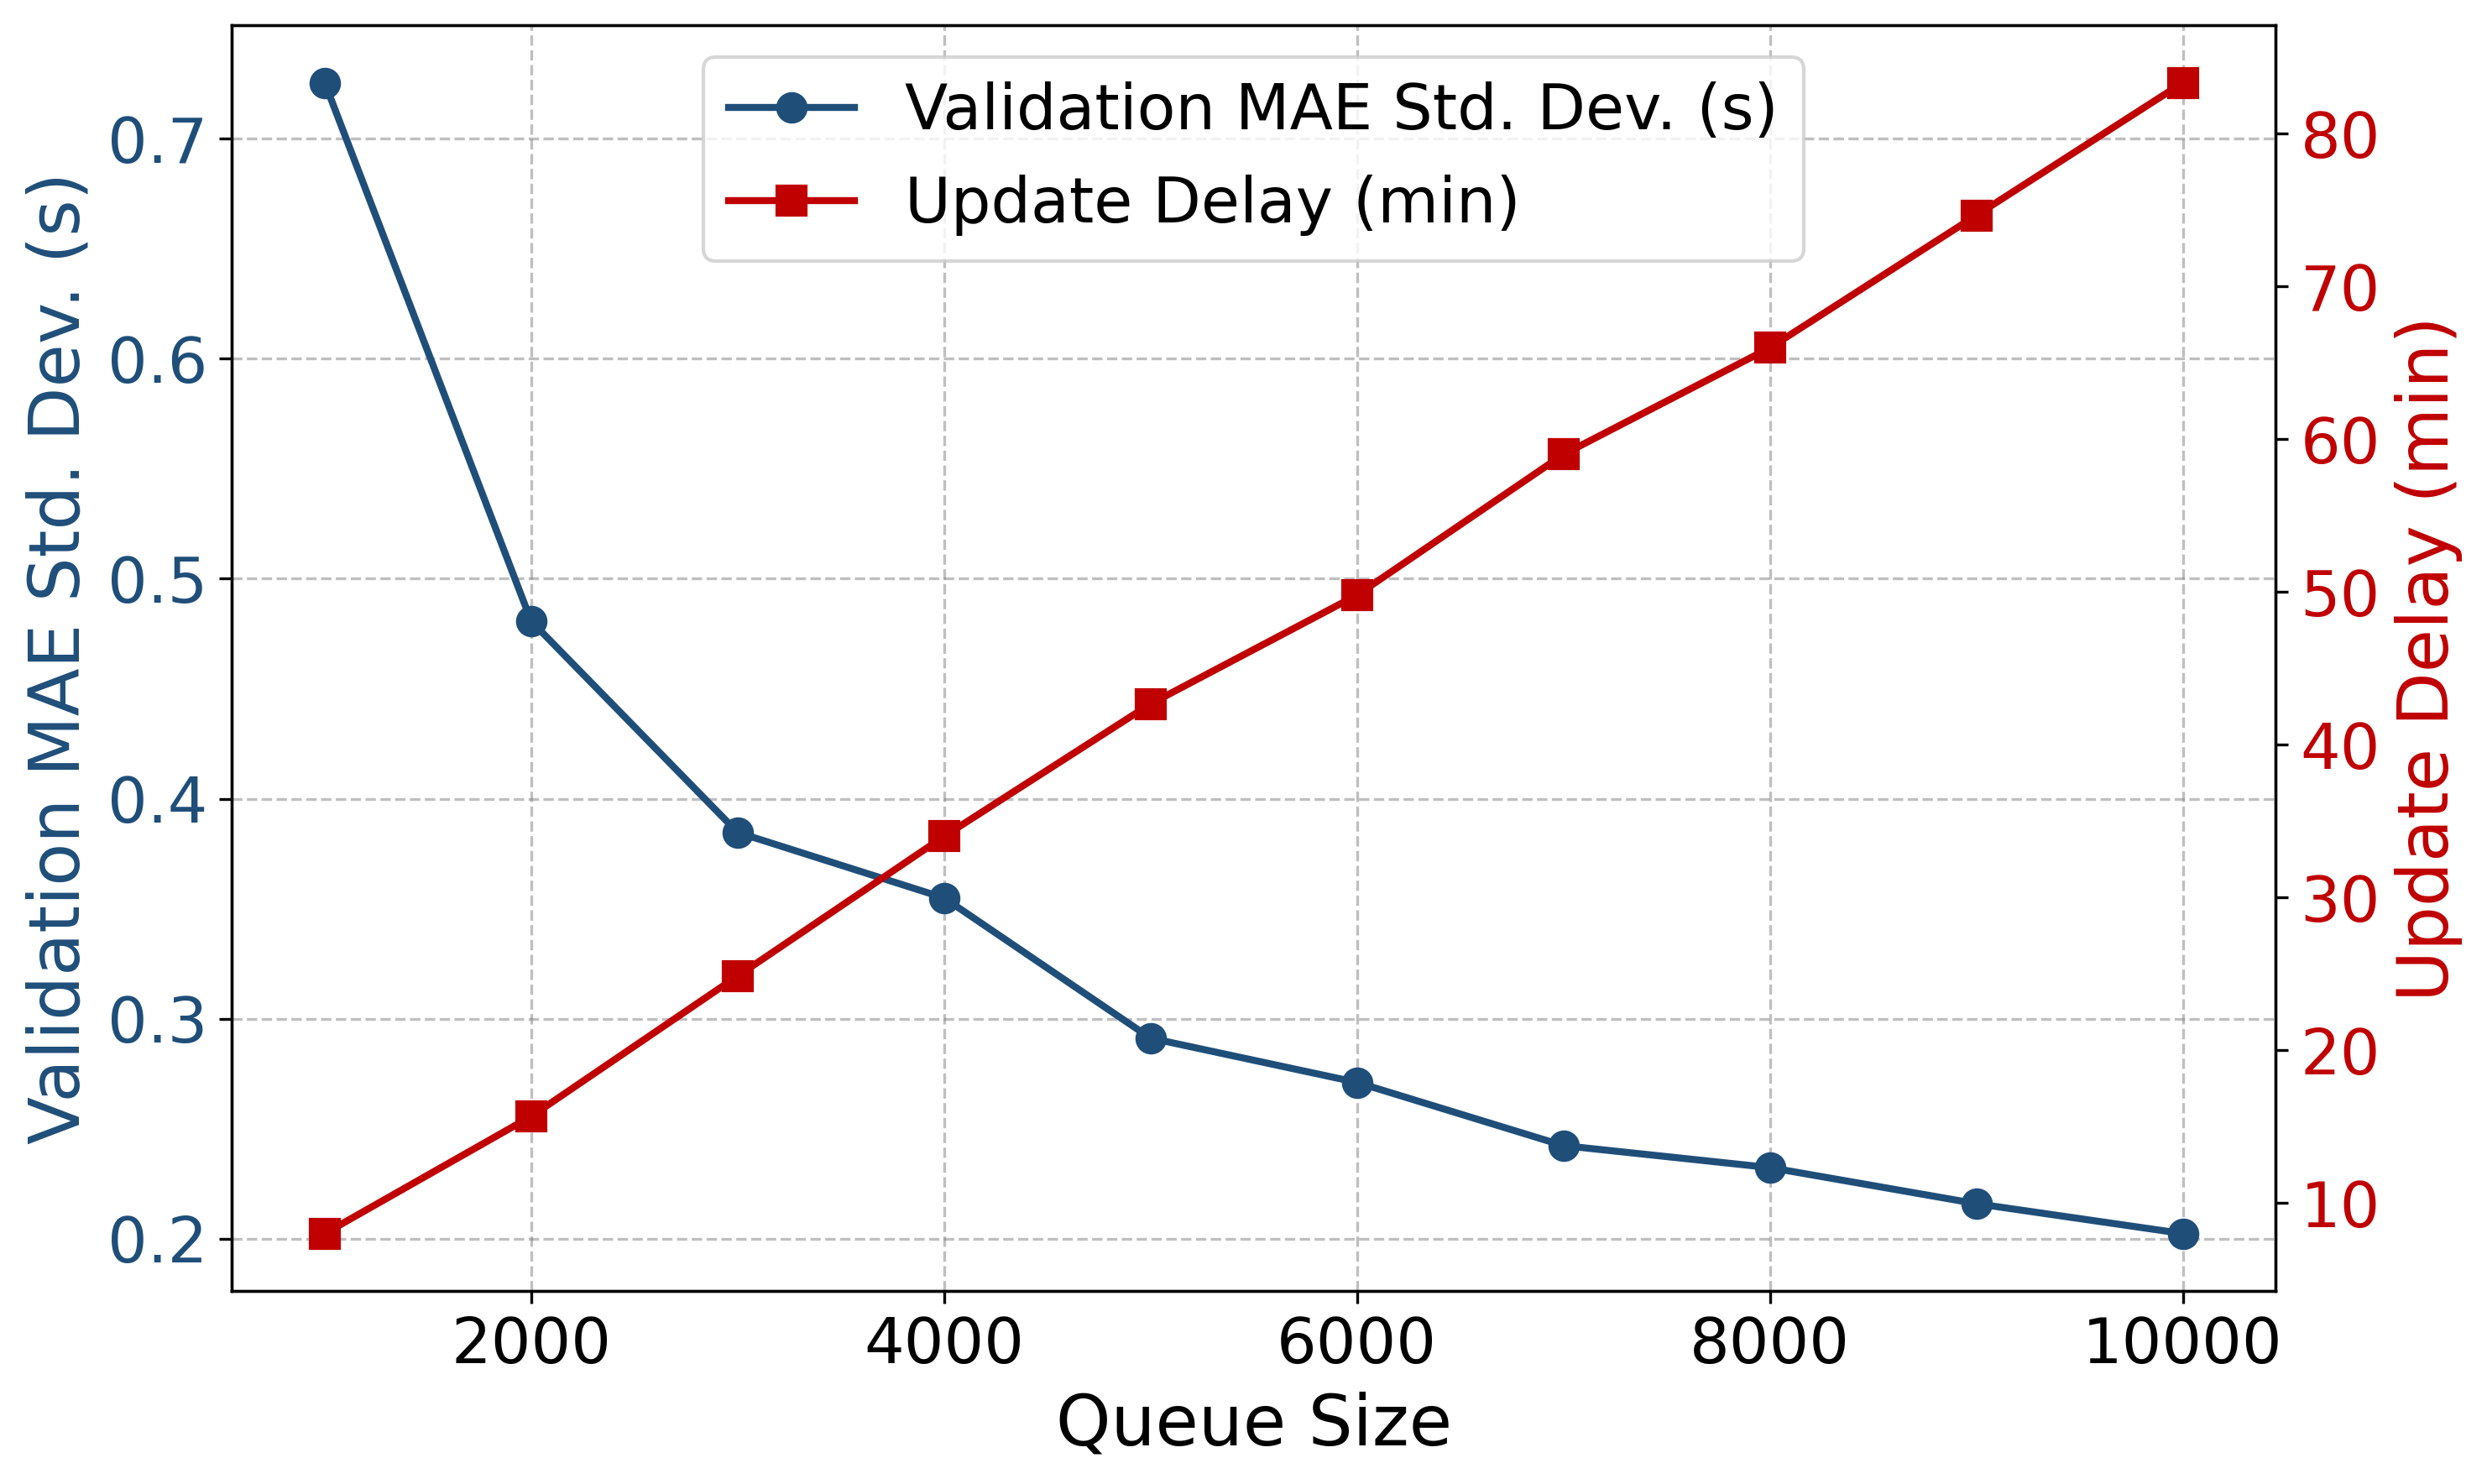
\includegraphics[width=\columnwidth]{figure/G4-2_queue_size_analysis.png}
\caption{Impact of queue size on MAE Std. Dev. (SEM) and Update Delay.}
\label{fig:G4-2}
\end{figure}

\begin{table*}[!t]
\centering
\caption{Average MAE During Periodic Local Adaptation (12 Rounds). H-ST-MBAN avoids catastrophic forgetting and achieves the lowest average MAE.}
\label{tab:finetune_accuracy}
\begin{tabular}{lccc}
\toprule
\textbf{Model} & \textbf{Global MAE (s)} & \textbf{Final MAE (s)} & \textbf{Average MAE (s) $\pm$ Std. Dev.} \\
\midrule
\textbf{H-ST-MBAN} & 58.39 & 17.58 & \textbf{20.33 $\pm$ 4.12} \\
FTT & 60.61 & 29.06 & 40.62 $\pm$ 10.02 \\
NGBoost & 42.26 & 43.86 & 42.26 $\pm$ 5.20 \\
LR & 51.87 & 54.77 & 51.87 $\pm$ 3.97 \\
LSTM & 52.38 & 53.58 & 52.06 $\pm$ 2.54 \\
TabPFN & 65.55 & 65.84 & 65.55 $\pm$ 0.55 \\
XGBoost & 71.44 & 72.65 & 71.44 $\pm$ 4.86 \\
CatBoost & 75.03 & 76.44 & 75.03 $\pm$ 5.85 \\
RF & 84.50 & 86.53 & 84.50 $\pm$ 8.15 \\
MLP & 64.01 & 85.74 & 100.91 $\pm$ 21.04 \\
ResNet & 51.89 & 79.44 & 103.58 $\pm$ 23.86 \\
GRU & 105.82 & 105.84 & 105.29 $\pm$ 6.45 \\
TabR & 56.69 & 90.64 & 106.38 $\pm$ 26.74 \\
\bottomrule
\end{tabular}
\end{table*}

\subsection{Periodic Local Adaptation Performance}
Figure~\ref{fig:G5} and Table~\ref{tab:finetune_accuracy} present the periodic local adaptation performance. As quantitatively summarized in Table~\ref{tab:finetune_accuracy}, H-ST-MBAN achieves the lowest average MAE of 20.33~\text{s}, outperforming all baseline models including the FTT model, which records 40.62~\text{s}. In addition, the MAE progression in Figure~\ref{fig:G5} visually demonstrates H-ST-MBAN's performance over the ML/NN baselines by preventing catastrophic forgetting. The proposed dual-model fine-tuning mechanism updates the local weights, maintaining a low error rate across continuous operation. In contrast, baseline models that lack this localized adaptation experience higher error over time as they fail to adapt to evolving traffic patterns. This performance advantage highlights the stability of combining GBDT-based boundary partition with deep temporal feature learning during online adaptation.

Validating the proposed edge fine-tuning strategy, Table~\ref{tab:finetune_accuracy} shows that H-ST-MBAN reduces its prediction error from a Global MAE of 58.39~s to a Final MAE of 17.58~s after fine-tuning. This improvement is accompanied by a low standard deviation of 4.12~s, indicating that the local adaptation process is stable. In contrast, standard deep learning baselines such as MLP, ResNet, and TabR exhibit performance degradation during the local fine-tuning phase. Due to local overfitting and gradient instability under resource-constrained conditions, their Average MAEs escalate beyond 100~s, reaching 100.91~s, 103.58~s, and 106.38~s for MLP, ResNet, and TabR, respectively. Similarly, their standard deviations soar past 20~s, yielding 21.04~s, 23.86~s, and 26.74~s. This numerical contrast reveals that these baseline architectures suffer from weight spiking and volatile optimization trajectories when updated with local edge queues. As a result, H-ST-MBAN maintains predictive reliability under dynamic traffic environments, whereas conventional neural network models fail to adapt. Meanwhile, traditional sequential baselines such as LSTM maintain a relatively stable error, yielding an Average MAE of 52.06~s, yet fail to approach the performance of H-ST-MBAN.

During the online adaptation process, the RSU edge node periodically accumulates vehicular state variables $X_v$ from incoming V2I content request packets into a local storage buffer. Under dynamic traffic environments, the inflow of outlier samples during this online training phase can induce gradient instability, which degrades deep learning weight configuration. H-ST-MBAN addresses this vulnerability by incorporating a steady-state filtering pre-processor at the RSU, which screens incoming state variables prior to gradient calculation. Compared to tree ensembles such as XGBoost that rely on fixed global weights and lack online model updates, H-ST-MBAN dynamically adjusts local weights using the local snapshot queue. Once the fine-tuning process completes, the updated model weights are applied to estimate the dwell duration, and the resulting prediction is transmitted to the caching scheduler to determine the prefetching queue configuration. This real-time sanitization phase prevents noisy updates, thereby preserving the structural stability of the globally trained prior weights.

During the periodic local adaptation process at the RSU edge node, standard deep learning baselines frequently exhibit performance degradation and sudden weight spikes in their loss curves. This instability during local adaptation originates from four primary structural causes under the dynamic vehicular network environment. First, local overfitting occurs due to data sparsity within the constrained local snapshot queue of size $Q=5000$, which fails to represent the broader traffic distribution. Second, standard neural networks experience catastrophic forgetting of globally acquired representations because they lack explicit regularization constraints to preserve pre-trained knowledge during local gradient steps. Third, unexpected traffic anomalies introduce extreme outlier samples, such as vehicles with dwell times exceeding 300 seconds, which leads to gradient pollution during backpropagation. Fourth, updating the entire parameter set through full fine-tuning under non-stationary edge traffic dynamics causes the optimization trajectory to diverge.

To overcome these vulnerabilities and stabilize the parameter update path, four corresponding mitigation strategies are required, which are structurally addressed by the H-ST-MBAN architecture. First, parameter-efficient fine-tuning or localized training of gating layers minimizes parameter drift, a mechanism realized by the gating fusion structure in H-ST-MBAN to control neural network weight variations. Second, global weight anchoring restricts the deviation between the local parameters and the globally pre-trained model weights. Third, applying a cosine annealing learning rate scheduler and enhanced weight decay prevents abrupt weight updates under noisy inputs. Fourth, the RSU utilizes a steady-state filtering pre-processor to sanitize the local queue before initiating gradient calculations. Once the fine-tuning iteration completes, the RSU computes the estimated vehicle dwell duration and transmits this value to the prefetching scheduler to configure the edge cache.

\begin{figure}[!t]
\centering
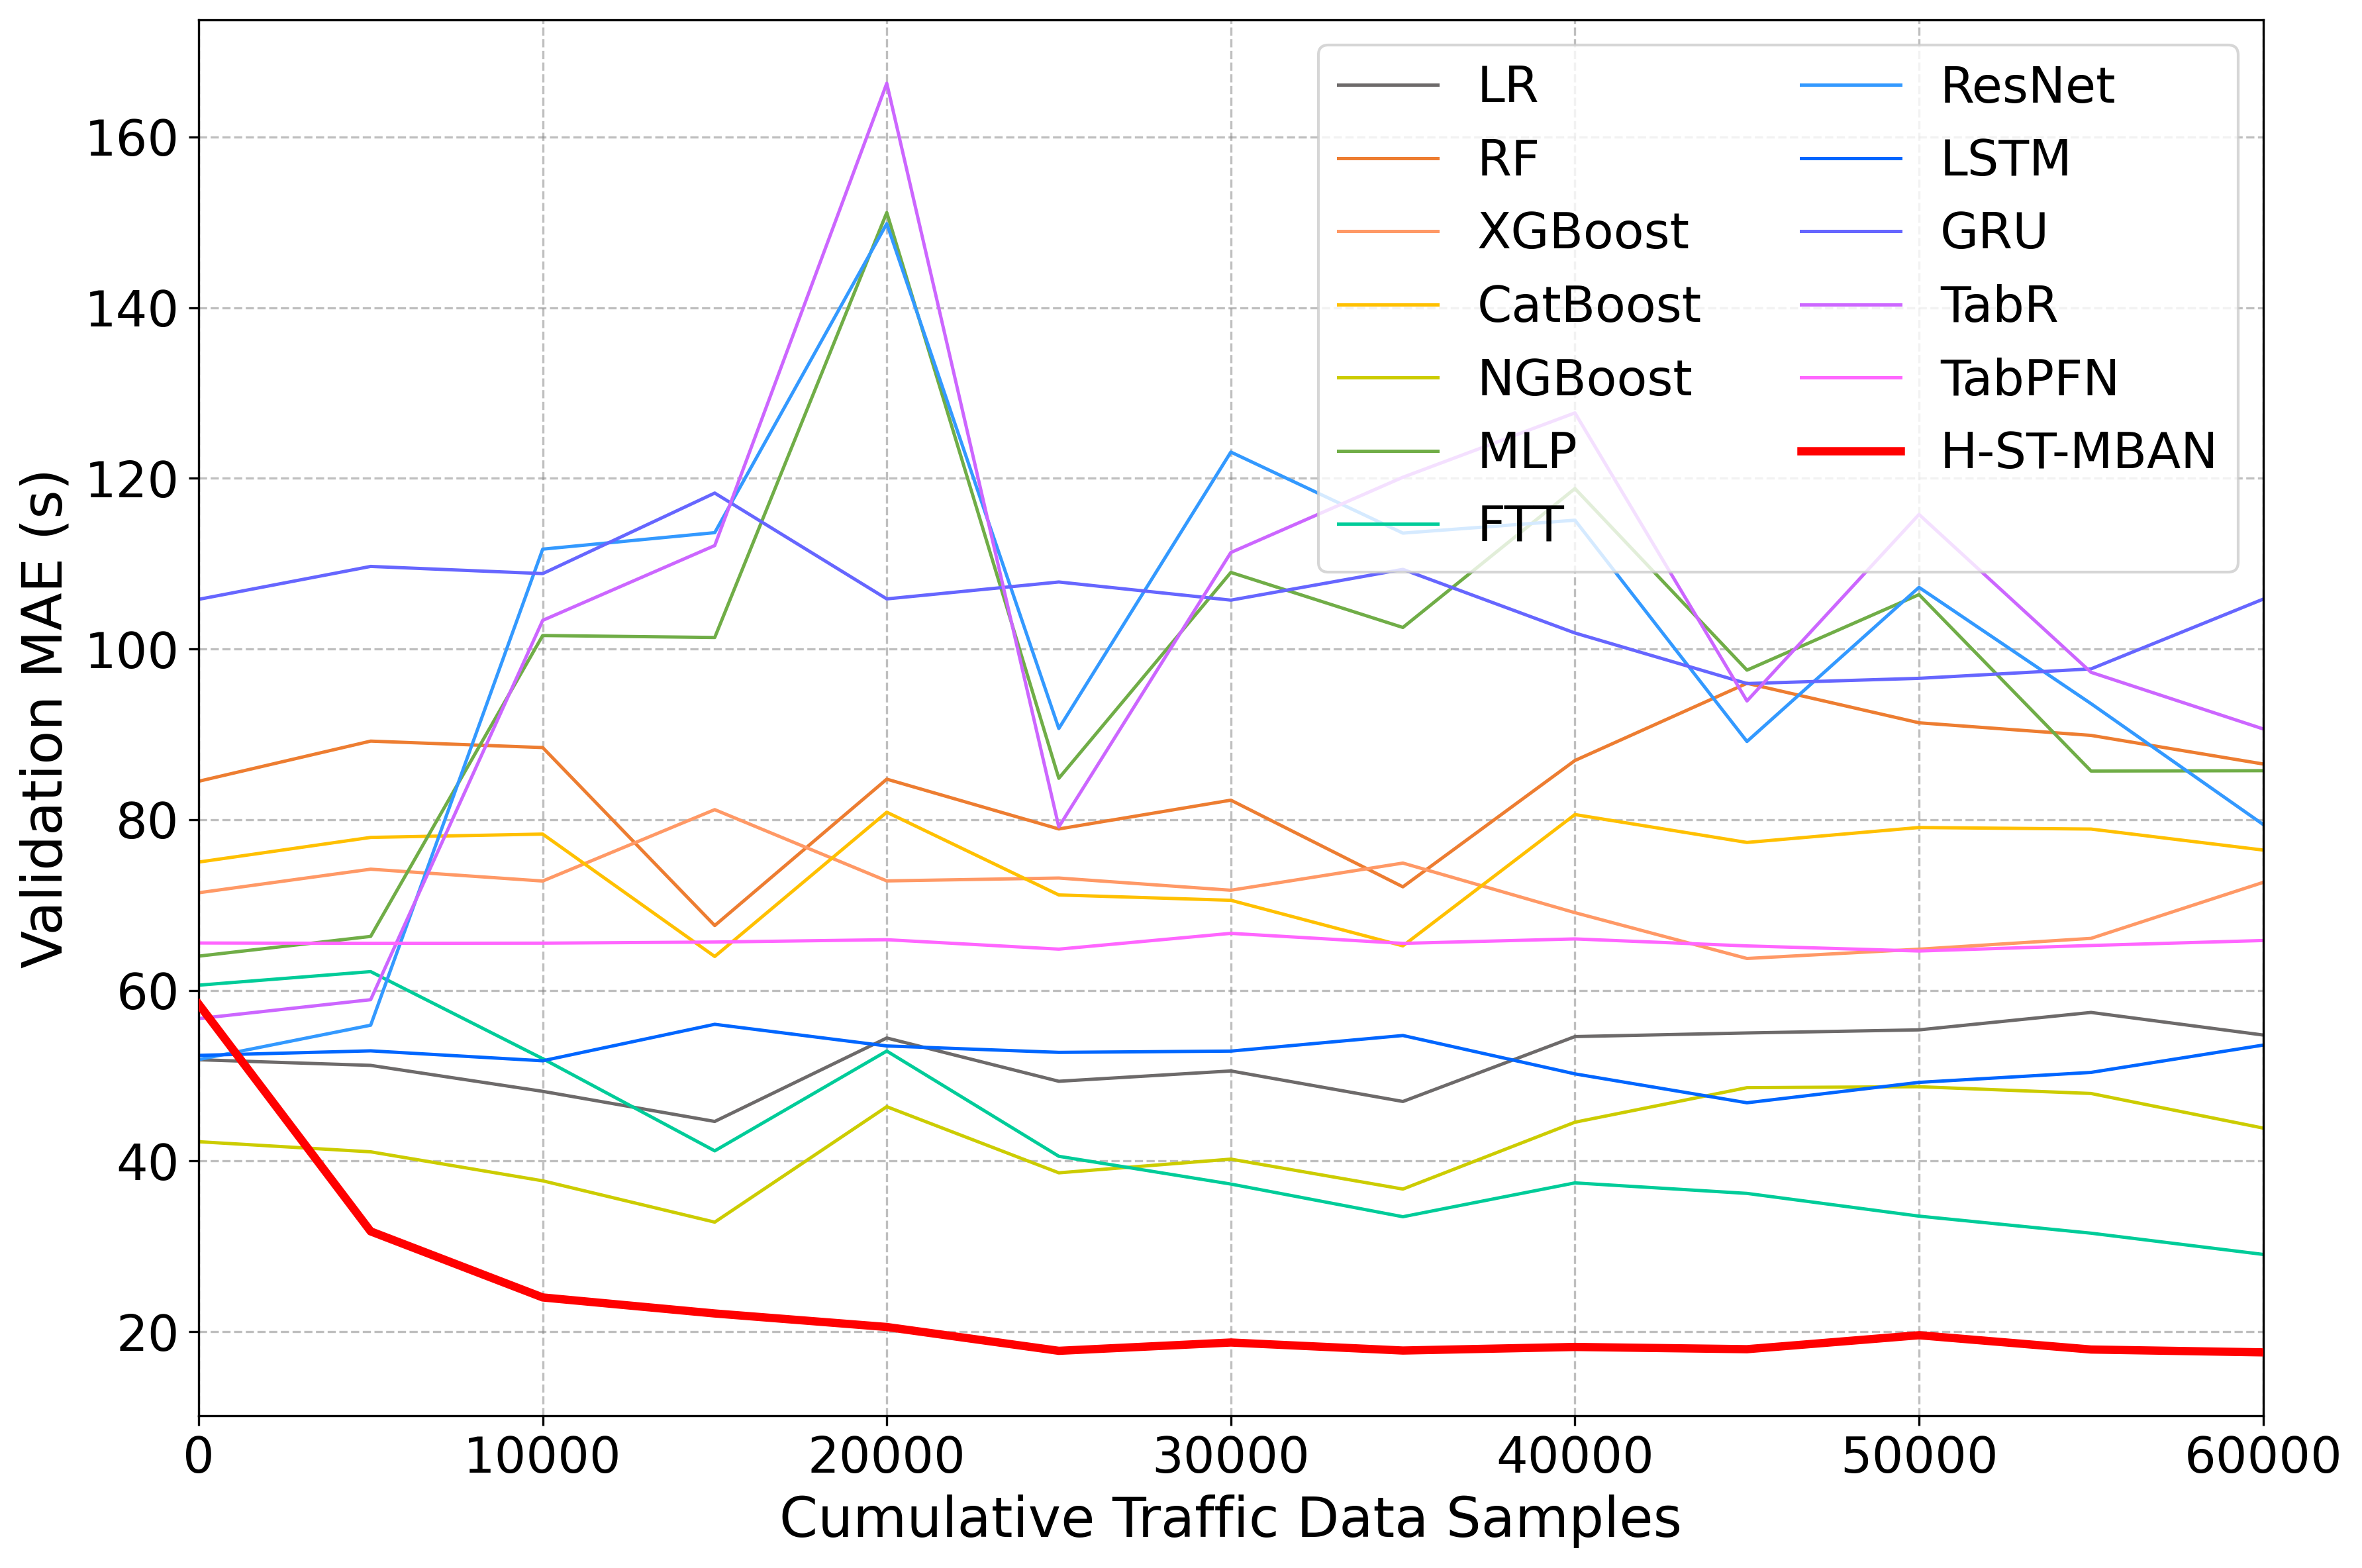
\includegraphics[width=\columnwidth]{figure/G5_baseline_comparison.png}
\caption{Cumulative validation MAE comparison of H-ST-MBAN against 12 ML/NN baselines under the optimal queue size Q=5000.}
\label{fig:G5}
\end{figure}

\begin{figure*}[!t]
\centering
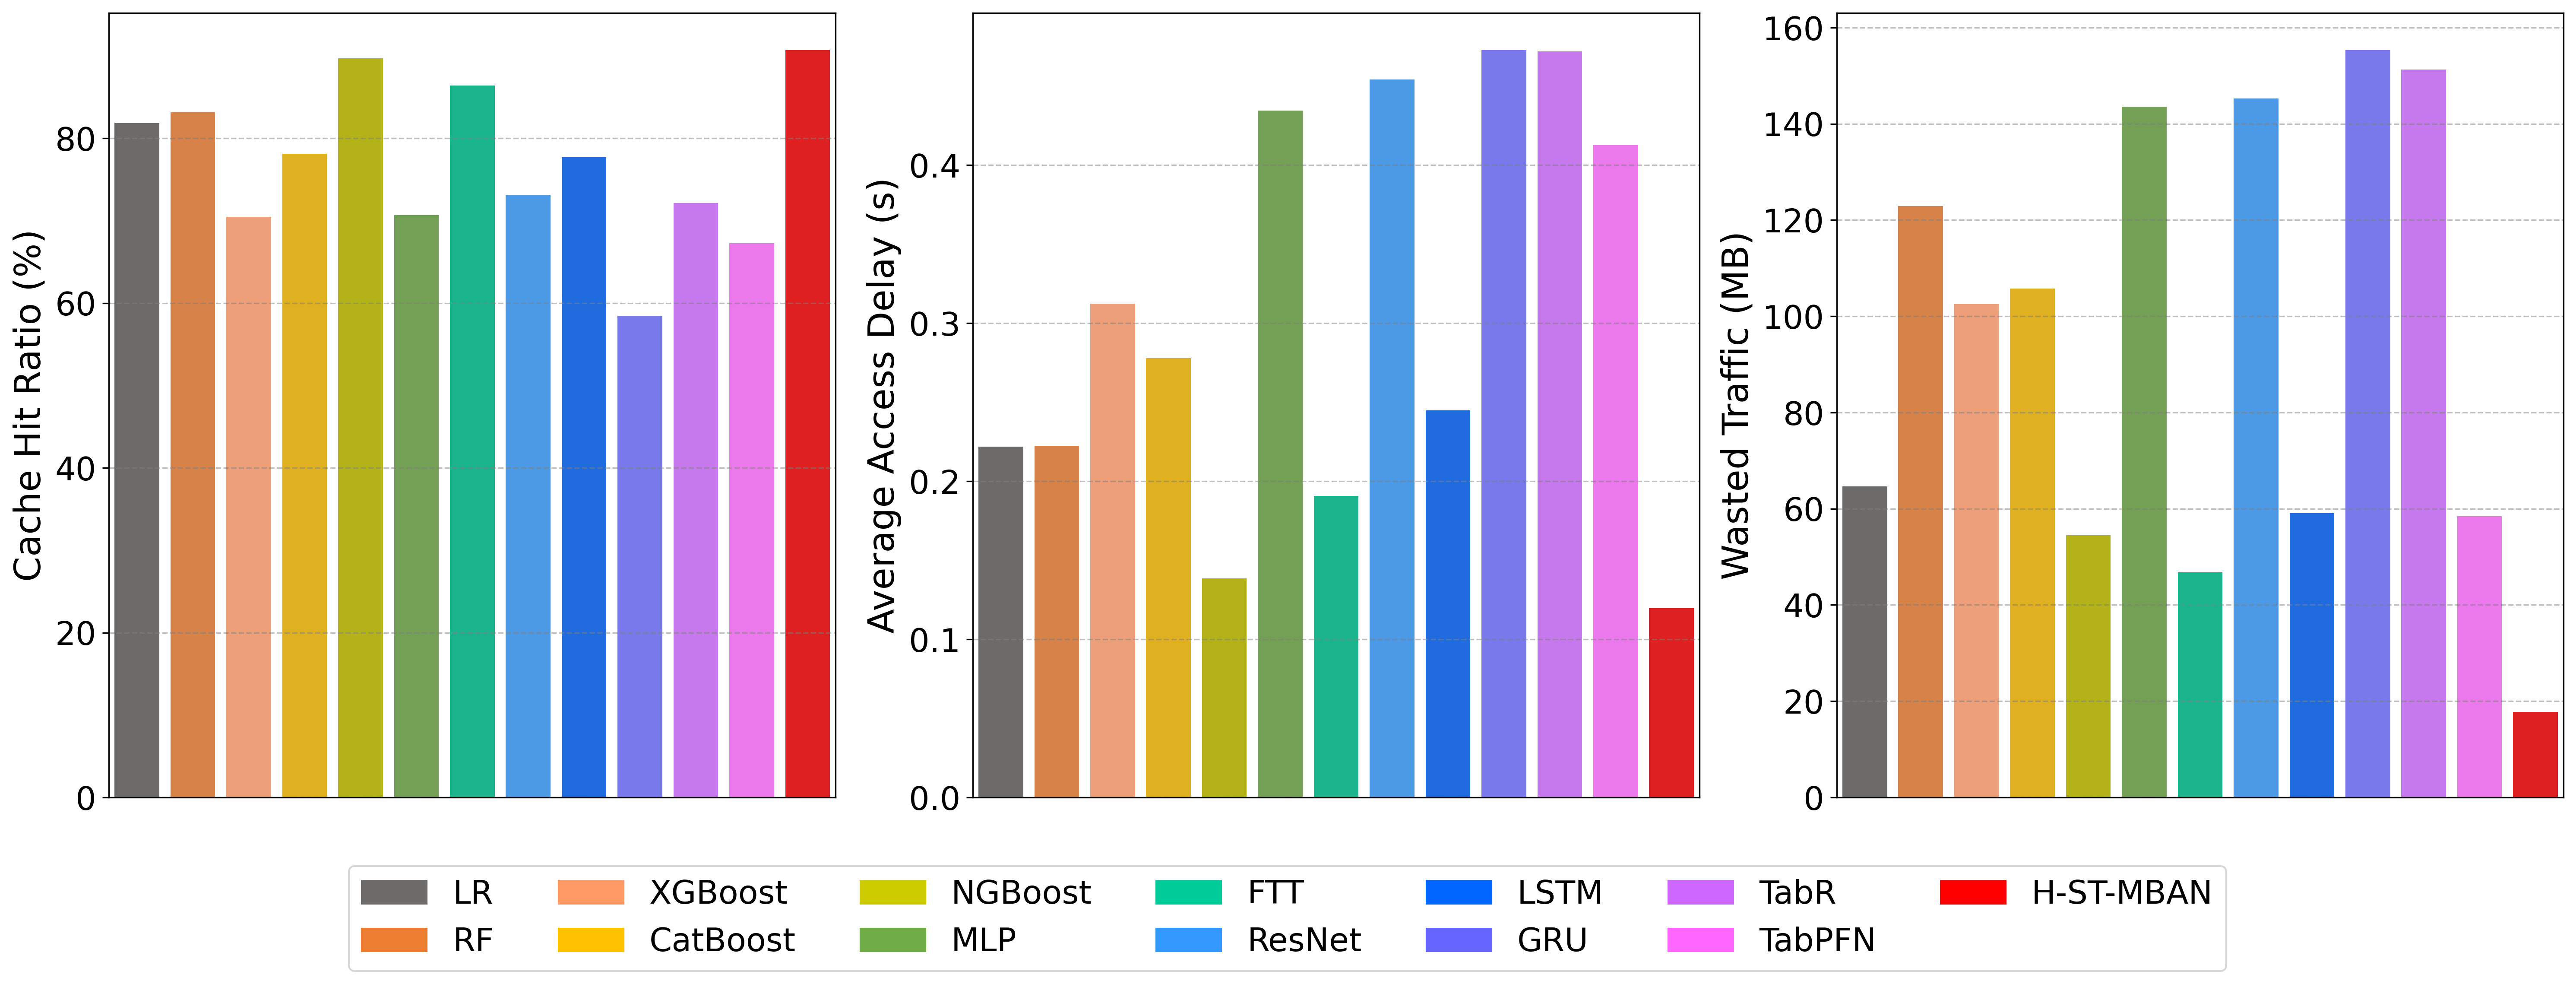
\includegraphics[width=\textwidth]{figure/G6_cache_metrics_avg.png}
\caption{Cache hit ratio, access delay, and wasted traffic comparing H-ST-MBAN against 12 baseline models.}
\label{fig:G6}
\end{figure*}

\begin{figure*}[!t]
\centering

\includegraphics[width=\textwidth]{figure/G7_cache_metrics_density.png}
\caption{Cache performance under varying vehicle densities, demonstrating the stability of H-ST-MBAN against complex spatial queuing dynamics.}
\label{fig:G7}
\end{figure*}

\subsection{Network Edge Caching Performance}
Figure~\ref{fig:G6} presents the average cache performance metrics, demonstrating that H-ST-MBAN achieves an average cache hit ratio of 90.70\% with a low average access delay of 0.1196~\text{s} and reduced wasted traffic of 17.70~\text{MB}. This performance advantage stems from the model's ability to accurately predict vehicle dwell times, allowing roadside units to proactively cache content with high precision. By improving cache placement accuracy, the proposed approach reduces user latency and minimizes redundant network traffic caused by incorrectly cached data, which translates to lower operational costs for bandwidth-constrained backhaul links. Furthermore, Figure~\ref{fig:G7} illustrates the impact of varying vehicle densities, showing that in the high-density interval of $(22.5, 25.0]~\text{veh/km/lane}$, H-ST-MBAN maintains a hit ratio of 91.64\% and stable access latency. Conversely, baseline models experience significant performance degradation due to their inability to capture the complex spatial queuing dynamics inherent in dense traffic. Overall, the sustained efficiency of H-ST-MBAN confirms that the network can maintain reliable service quality and stable caching performance even during complex congestion patterns at peak traffic hours.

The integration of accurate dwell time forecasting directly dictates the overall efficiency of edge caching mechanisms. Specifically, the low MAE accurately matches the dwell time prediction to prevent unnecessary content eviction from the constrained local storage. In conjunction with this predictive precision, the dynamically adaptive coefficient $\eta(t)$ acts as a safety margin buffer against sudden wireless bandwidth fluctuations. By absorbing these transient physical layer anomalies, the proactive scheduling algorithm ensures that the edge infrastructure downloads precisely the deliverable volume of data. Consequently, this synergistic approach eliminates premature caching termination and over-prefetching waste, ultimately achieving a 90.7\% average Cache Hit Ratio across diverse operational environments.
\section{Conclusion} \label{sec:conclusion}
In this paper, we proposed H-ST-MBAN, a deterministic regression model for dwell-time prediction in CCVNs.
To address complex traffic patterns and inference latency, H-ST-MBAN adopts a hybrid residual regression architecture.
By establishing an XGBoost base prediction and learning the spatio-temporal residual errors through semantically partitioned branch encoders fused via MHA, the model captures traffic dynamics without additional computational overhead.
Evaluations using the SUMO traffic simulator demonstrated that H-ST-MBAN achieves the lowest prediction error compared to 12 baseline models, yielding a MAE of 44.32~s and robust stability against traffic outliers.
Ablation studies confirmed that the GBDT prior stream, multi-branch attention structure, and deep residual decoder contribute to maintaining prediction accuracy and convergence speed.
The integration of physical traffic constraints with non-linear neural mapping establishes a practical methodology for decentralized edge intelligence in intelligent transportation systems.

Network-level simulations demonstrated that H-ST-MBAN supports proactive caching by reducing access delay and wasted traffic.
When vehicle density increases, traffic congestion extends the vehicle dwell time within the intersection coverage of the road-side unit.
This extended residency duration provides the edge node with sufficient time to prefetch and cache requested content chunks, enabling the system to maintain a cache hit ratio of 91.64\% under dense traffic conditions, which exceeds the average hit ratio of 90.70\%.
Theoretical hardware profiling verified that the proposed fine-tuning strategy is computationally feasible on standard RSU edge devices, requiring only 1.38~M parameters and 47.69~MB of peak memory.
This low-overhead feasibility allows the predictive framework to function independently and mitigate catastrophic forgetting through continuous local adaptation, circumventing centralized processing bottlenecks without overloading the V2I uplink capacity.
In future work, we plan to extend H-ST-MBAN by integrating federated learning across multiple RSUs, enabling collaborative adaptation to city-scale traffic anomalies while preserving vehicle privacy.

% \section*{Acknowledgment} This work was supported by the National Research Foundation of Korea (NRF) grant funded by the Korea government (MSIT) (No. 2022R1A2C1010121).

\bibliographystyle{IEEEtran}
\begin{thebibliography}{99}
\bibitem{ericsson2023}
Ericsson, ``Ericsson Mobility Report,'' \emph{Ericsson}, Stockholm, Sweden, 2023. [Online]. Available: https://www.ericsson.com/en/reports-and-papers/mobility-report

\bibitem{wang2017}
Meng Wang, Jun Wu, Gaolei Li, Jianhua Li, Qiang Li, and Shen Wang, ``Toward mobility support for information-centric IoV in smart city using fog computing,'' \emph{2017 IEEE International Conference on Smart Energy Grid Engineering (SEGE)}, Oshawa, ON, Canada, pp. 357--361, 2017.%, doi: 10.1109/SEGE.2017.8052825.

\bibitem{nam2025}
Youngju Nam, Hyeonseok Choi, and Euisin Lee, ``Content Storage Management and Precaching Scheme in Content-Centric-Network-Based Internet of Vehicles,'' \emph{IEEE Internet of Things Journal}, vol. 12, no. 9, pp. 12927--12947, 2025.%, doi: 10.1109/JIOT.2024.3522322.

\bibitem{su2018}
Zhou Su, Yilong Hui, Qichao Xu, Tingting Yang, Jianyi Liu, and Yunjian Jia, ``An Edge Caching Scheme to Distribute Content in Vehicular Networks,'' \emph{IEEE Transactions on Vehicular Technology}, vol. 67, no. 6, pp. 5346--5356, 2018.%, doi: 10.1109/TVT.2018.2824345.

\bibitem{huang2019}
Wanying Huang, Tian Song, Yating Yang, and Yu Zhang, ``Cluster-Based Cooperative Caching With Mobility Prediction in Vehicular Named Data Networking,'' \emph{IEEE Access}, vol. 7, pp. 23442--23458, 2019.%, doi: 10.1109/ACCESS.2019.2897747.

\bibitem{feng2023}
Biqian Feng, Chenyuan Feng, Daquan Feng, Yongpeng Wu, and Xiang-Gen Xia, ``Proactive Content Caching Scheme in Urban Vehicular Networks,'' \emph{IEEE Transactions on Communications}, vol. 71, no. 7, pp. 4165--4180, 2023.%, doi: 10.1109/TCOMM.2023.3277530.

\bibitem{wang2025}
Chenglong Wang, Jun Peng, Lin Cai, Weirong Liu, Ziyu Zhao, Hu He, and Zhiwu Huang, ``Mobility and Context-Aware Precaching Strategy Using Spatial-Temporal Informer for Vehicular Service,'' \emph{IEEE Internet of Things Journal}, vol. 12, no. 11, pp. 16053--16066, 2025.%, doi: 10.1109/JIOT.2025.3530699.

\bibitem{cheng2025}
Jinguo Cheng, Ke Li, Yuxuan Liang, Lijun Sun, Junchi Yan, and Yuankai Wu, ``Rethinking Urban Mobility Prediction: A Multivariate Time Series Forecasting Approach,'' \emph{IEEE Transactions on Intelligent Transportation Systems}, vol. 26, no. 2, pp. 2543--2557, 2025.%, doi: 10.1109/TITS.2024.3498054.

\bibitem{jiang2024}
Kai Jiang, Yue Cao, Yujie Song, Huan Zhou, Shaohua Wan, and Xu Zhang, ``Asynchronous Federated and Reinforcement Learning for Mobility-Aware Edge Caching in IoV,'' \emph{IEEE Internet of Things Journal}, vol. 11, no. 9, pp. 15334--15347, 2024.%, doi: 10.1109/JIOT.2023.3349255.

\bibitem{yu2024}
Genghua Yu, Jian Wu, Rui Liu, Yixin He, Zhigang Chen, and Jianping Pan, ``Joint Cooperative Caching and UAV Trajectory Optimization Based on Mobility Prediction in the Internet of Connected Vehicles,'' \emph{IEEE Transactions on Intelligent Transportation Systems}, vol. 25, no. 11, pp. 17392--17406, 2024.%, doi: 10.1109/TITS.2024.3429305.

\bibitem{aung2023}
Nyothiri Aung, Sahraoui Dhelim, Liming Chen, Abderrahmane Lakas, Wenyin Zhang, Huansheng Ning, Souleyman Chaib, and Mohand Tahar Kechadi, ``VeSoNet: Traffic-Aware Content Caching for Vehicular Social Networks Using Deep Reinforcement Learning,'' \emph{IEEE Transactions on Intelligent Transportation Systems}, vol. 24, no. 8, pp. 8638--8649, 2023.%, doi: 10.1109/TITS.2023.3250320.

\bibitem{su2017}
Zhou Su, Yilong Hui, and Qing Yang, ``The Next Generation Vehicular Networks: A Content-Centric Framework,'' \emph{IEEE Wireless Communications}, vol. 24, no. 1, pp. 60--66, 2017.%, doi: 10.1109/MWC.2017.1600195WC.

\bibitem{li2017}
Zhuo Li, Yutong Chen, Deliang Liu, and Xiang Li, ``Performance analysis for an enhanced architecture of IoV via Content-Centric Networking,'' \emph{EURASIP Journal on Wireless Communications and Networking}, vol. 2017, no. 1, 2017.%, doi: 10.1186/S13638-017-0905-4.

\bibitem{khan2018}
Irfanullah Khan, Tiankui Zhang, Xiaogeng Xu, Siyang Shan, Adil Khan, and Shabeer Ahmad, ``Priority-based Content Dissemination in Content Centric Vehicular Networks,'' \emph{2018 2nd IEEE Advanced Information Management, Communicates, Electronic and Automation Control Conference (IMCEC)}, Xi'an, China, pp. 1162--1166, 2018.%, doi: 10.1109/IMCEC.2018.8469332.

\bibitem{khan2025}
Sajjad Ahmad Khan, Huhnkuk Lim, and Shehzad Ashraf Chaudhry, ``Adaptive Data Forwarding Scheme for Diverse Infotainment Services in Vehicular Named Data Networking,'' \emph{IEEE Transactions on Vehicular Technology}, vol. 74, no. 5, pp. 8012--8022, 2025.%, doi: 10.1109/TVT.2024.3524122.

\bibitem{lim2025}
Huhnkuk Lim, ``Toward Infotainment Services in Vehicular Named Data Networking: A Comprehensive Framework Design and Its Realization,'' \emph{IEEE Transactions on Intelligent Transportation Systems}, vol. 26, no. 2, pp. 2793--2810, 2025.%, doi: 10.1109/TITS.2024.3489574.

\bibitem{khan2025_2}
Azan Ali Khan, Basharat Hussain, Muhammad Islam, Maryam M. Al Dabel, and Ali Kashif Bashir, ``Optimizing Content Cache With Vehicular Edge Computing: A Deep Federated Learning-Based Novel Predictive Study,'' \emph{IEEE Transactions on Consumer Electronics}, vol. 71, no. 2, pp. 6069--6079, 2025.%, doi: 10.1109/TCE.2025.3571029.

\bibitem{cao2025}
Tengfei Cao, Nianqing Zhang, Xiaoying Wang, and Jianqiang Huang, ``Mobility-Aware Cooperative Caching in Vehicular Edge Computing Based on Federated Distillation and Deep Reinforcement Learning,'' \emph{IEEE Transactions on Network Science and Engineering}, pp. 1--17, 2025.%, doi: 10.1109/TNSE.2025.3571902.

\bibitem{wang2025_2}
Yali Wang and Shouhao Li, ``Federated Learning-based Vehicle Edge Caching Optimization Strategy,'' \emph{2025 IEEE 6th International Conference on Pattern Recognition and Machine Learning (PRML)}, Chongqing, China, pp. 285--290, 2025.%, doi: 10.1109/PRML66062.2025.11160265.

\bibitem{xie2026}
Yaqin Xie, Chengshuai Zhou, Zhongyu Liu, Yu Zhang, Jianyue Zhu, and Junmin Wu, ``Research on Cache Placement Optimization and Popularity-Based Content Prefetching Strategy in LEO Satellite Networks,'' \emph{IEEE Transactions on Green Communications and Networking}, vol. 10, pp. 50--62, 2026.%, doi: 10.1109/TGCN.2025.3570489.

\bibitem{liao2025}
Zhuofan Liao, Pang Liu, Bin Zheng, and XiaoYong Tang, ``Context-Aware Proactive Edge Caching for Vehicular Edge Computing Based on Asynchronous Federated Learning,'' \emph{IEEE Internet of Things Journal}, vol. 12, no. 13, pp. 23195--23206, 2025.%, doi: 10.1109/JIOT.2025.3552682.

\bibitem{liu2024}
Rui Liu and Jianping Pan, ``CRS: A Privacy-Preserving Two-Layered Distributed Machine Learning Framework for IoV,'' \emph{IEEE Internet of Things Journal}, vol. 11, no. 1, pp. 1080--1095, 2024.%, doi: 10.1109/JIOT.2023.3287799.

\bibitem{yang2024}
Qin Yang and Sang-Jo Yoo, ``Hierarchical Reinforcement Learning-Based Routing Algorithm With Grouped RSU in Urban VANETs,'' \emph{IEEE Transactions on Intelligent Transportation Systems}, vol. 25, no. 8, pp. 10131--10146, 2024.%, doi: 10.1109/TITS.2024.3353258.

\bibitem{gopal2023}
Govind R. Gopal, Jie Chen, William J. Hillery, Jun Tan, Serdar Özen, and Qiping Zhu, ``Wireless Channel Scenario Identification Using Convolutional Neural Networks,'' \emph{2023 IEEE 97th Vehicular Technology Conference (VTC2023-Spring)}, Florence, Italy, pp. 1--5, 2023.%, doi: 10.1109/VTC2023-Spring57618.2023.10200552.

\bibitem{hasan2024}
Mohammad Kamrul Hasan, Nusrat Jahan, Mohd Zakree Ahmad Nazri, Shayla Islam, Muhammad Attique Khan, Ahmed Ibrahim Alzahrani, Nasser Alalwan, and Yunyoung Nam, ``Federated Learning for Computational Offloading and Resource Management of Vehicular Edge Computing in 6G-V2X Network,'' \emph{IEEE Transactions on Consumer Electronics}, vol. 70, no. 1, pp. 3827--3847, 2024.%, doi: 10.1109/TCE.2024.3357530.

\bibitem{zhang2024}
Xinran Zhang, Zheng Chang, Tao Hu, Weilong Chen, Xin Zhang, and Geyong Min, ``Vehicle Selection and Resource Allocation for Federated Learning-Assisted Vehicular Network,'' \emph{IEEE Transactions on Mobile Computing}, vol. 23, no. 5, pp. 3817--3829, 2024.%, doi: 10.1109/TMC.2023.3283295.

\bibitem{xu2024}
Bo Xu, Haitao Zhao, Haotong Cao, Xiaozhen Lu, and Hongbo Zhu, ``Joint Contract Design and Task Reorganization for Semi-Decentralized Federated Edge Learning in Vehicular Networks,'' \emph{IEEE Transactions on Vehicular Technology}, vol. 73, no. 7, pp. 10539--10553, 2024.%, doi: 10.1109/TVT.2024.3364515.

\bibitem{park2024}
Soohyun Park, Chanyoung Park, Soyi Jung, Minseok Choi, and Joongheon Kim, ``Age-of-Information Aware Caching and Delivery for Infrastructure-Assisted Connected Vehicles,'' \emph{IEEE Transactions on Vehicular Technology}, vol. 73, no. 7, pp. 10681--10696, 2024.%, doi: 10.1109/TVT.2024.3384952.

\bibitem{cox1958}
D. R. Cox, ``The regression analysis of binary sequences,'' \emph{Journal of the Royal Statistical Society: Series B (Methodological)}, vol. 20, no. 2, pp. 215--232, 1958.%, doi: 10.1111/j.2517-6161.1958.tb00292.x.

\bibitem{breiman2001}
L. Breiman, ``Random forests,'' \emph{Machine Learning}, vol. 45, no. 1, pp. 5--32, 2001.%, doi: 10.1023/A:1010933404324.

\bibitem{chen2016}
T. Chen and C. Guestrin, ``XGBoost: A scalable tree boosting system,'' \emph{Proceedings of the 22nd ACM SIGKDD International Conference on Knowledge Discovery and Data Mining}, San Francisco, CA, USA, pp. 785--794, 2016.%, doi: 10.1145/2939672.2939785.

\bibitem{prokhorenkova2018}
L. Prokhorenkova, G. Gusev, A. Vorobev, A. V. Dorogush, and A. Gulin, ``CatBoost: unbiased boosting with categorical features,'' \emph{Advances in Neural Information Processing Systems}, Montr\'eal, QC, Canada, pp. 6638--6648, 2018.%, doi: 10.48550/arXiv.1706.09516.

\bibitem{duan2020}
T. Duan, A. Anand, D. Y. Ding, K. K. Thai, S. Schuler, A. Y. Ng, and A. Schuler, ``NGBoost: Natural gradient boosting for probabilistic prediction,'' \emph{International Conference on Machine Learning}, Vienna, Austria, pp. 2690--2700, 2020.%, doi: 10.48550/arXiv.1910.03225.

\bibitem{rumelhart1986}
D. E. Rumelhart, G. E. Hinton, and R. J. Williams, ``Learning representations by back-propagating errors,'' \emph{Nature}, vol. 323, no. 6088, pp. 533--536, 1986.%, doi: 10.1038/323533a0.

\bibitem{gorishniy2021}
Y. Gorishniy, I. Rubachev, V. Khrulkov, and A. Babenko, ``Revisiting Deep Learning Models for Tabular Data,'' \emph{Advances in Neural Information Processing Systems}, Virtual Event, pp. 18932--18943, 2021.%, doi: 10.48550/arXiv.2106.11959.

\bibitem{he2016}
K. He, X. Zhang, S. Ren, and J. Sun, ``Deep residual learning for image recognition,'' \emph{Proceedings of the IEEE Conference on Computer Vision and Pattern Recognition (CVPR)}, Las Vegas, NV, USA, pp. 770--778, 2016.%, doi: 10.1109/CVPR.2016.90.

\bibitem{hochreiter1997}
S. Hochreiter and J. Schmidhuber, ``Long short-term memory,'' \emph{Neural Computation}, vol. 9, no. 8, pp. 1735--1780, 1997.%, doi: 10.1162/neco.1997.9.8.1735.

\bibitem{cho2014}
K. Cho, B. Van Merri\"enboer, C. Gulcehre, D. Bahdanau, F. Bougares, H. Schwenk, and Y. Bengio, ``Learning phrase representations using RNN encoder-decoder for statistical machine translation,'' \emph{Proceedings of the 2014 Conference on Empirical Methods in Natural Language Processing (EMNLP)}, Doha, Qatar, pp. 1724--1734, 2014.%, doi: 10.3115/v1/D14-1179.

\bibitem{gorishniy2024}
Y. Gorishniy, I. Rubachev, N. Kartashev, D. Shlenskii, A. Kotelnikov, and A. Babenko, ``TabR: Tabular Deep Learning Meets Nearest Neighbors,'' \emph{The Twelfth International Conference on Learning Representations}, Vienna, Austria, 2024.%, doi: 10.48550/arXiv.2307.14338.

\bibitem{hollmann2023}
N. Hollmann, S. M\"uller, K. Eggensperger, and F. Hutter, ``TabPFN: A Transformer That Solves Small Tabular Classification Problems in a Second,'' \emph{The Eleventh International Conference on Learning Representations}, Kigali, Rwanda, 2023.%, doi: 10.48550/arXiv.2207.01848.

\bibitem{office2021}
Intelligent Transportation Systems Joint Program Office, ``ITS Standards Program: Strategic Plan 2021--2026,'' \emph{U.S. Department of Transportation}, 2021.

% \bibitem{xu2025}
% Liang Xu, Kaitao Meng, Deshi Li, Rui Wang, and Lele Cong, ``Adaptive Video Segment Pre-Caching With Varying Travel Duration for Internet of Vehicles,'' \emph{IEEE Internet of Things Journal}, 2025, doi: 10.1109/JIOT.2025.3587768.

% \bibitem{hu2018}
% Jie Hu, Li Shen, and Gang Sun, ``Squeeze-and-Excitation Networks,'' \emph{Proceedings of the IEEE Conference on Computer Vision and Pattern Recognition (CVPR)}, Salt Lake City, UT, USA, pp. 7132--7141, 2018, doi: 10.1109/CVPR.2018.00745.

% \bibitem{vaswani2017}
% Ashish Vaswani, Noam Shazeer, Niki Parmar, Jakob Uszkoreit, Llion Jones, Aidan N. Gomez, Lukasz Kaiser, and Illia Polosukhin, ``Attention Is All You Need,'' \emph{Advances in Neural Information Processing Systems}, Long Beach, CA, USA, pp. 5998--6008, 2017, doi: 10.48550/arXiv.1706.03762.

\end{thebibliography}

\begin{IEEEbiography}[{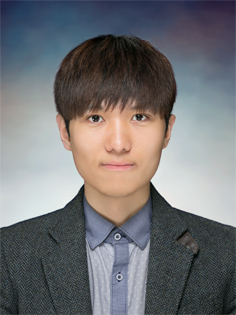
\includegraphics[width=1in,height=1.25in,clip,keepaspectratio]{./photo/YoungjuNam.jpg}}]
{Youngju Nam} received the B.S., M.S., and Ph.D. degrees from the School of Information and Communication Engineering, Chungbuk National University, Cheongju, South Korea, in 2017, 2019, and 2023, respectively. He joined the School of Software, Kunsan National University, in 2024, where he is currently working as an Assistant Professor. His research interests include computer communication and networking, wireless sensor networks, content-centric vehicular networks, content precaching, optimization, and social networks.
\end{IEEEbiography}

\begin{IEEEbiography}[{
\includegraphics[width=1in,height=1.25in,clip,keepaspectratio]{./photo/YongjeShin.jpg}}]
{Yongje Shin} received the B.S., M.S., and Ph.D. degrees from the School of Information and Communication Engineering, Chungbuk National University, Cheongju, South Korea, in 2016, 2018, and 2022, respectively. From 2022 to 2025, he was a Postdoctoral Researcher with the Research Institute for Computer and Information Communication, Chungbuk National University. Since March 2026, he has been an Assistant Professor with the School of Smart IT, Semyung University, Jecheon, South Korea. His research interests include computer communication and networking, wireless sensor networks, vehicular ad hoc networks (VANETs), mobility management, social intelligence networks, and AI-based intelligent networking systems.
\end{IEEEbiography}

\begin{IEEEbiography}[{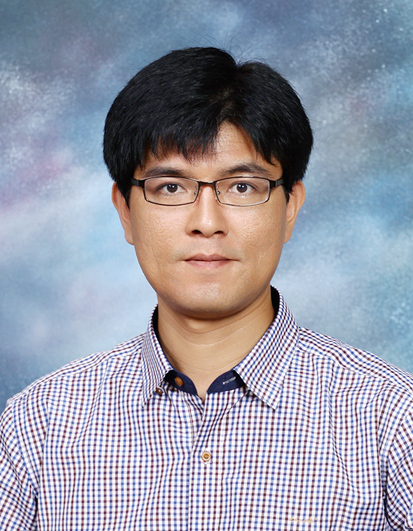
\includegraphics[width=1in,height=1.25in,clip,keepaspectratio]{./photo/EuisinLee.jpg}}]
{Euisin Lee} received the B.S., M.S., and Ph.D. degrees in computer engineering from Chungnam National University, Daejeon, South Korea, in 2005, 2007, and 2012, respectively. He studied as a Postdoctoral Researcher with the Department of Computer Science, University of California at Los Angeles, from 2012 to 2014. He joined the School of Information and Communication Engineering, Chungbuk National University, in 2014, where he is currently working as a Professor. His research interests include computer communication and networking, routing, multicasting, mobility management, location service, QoS (real-time and reliability) in mobile ad hoc networks (MANETs), wireless sensor networks (WSNs), vehicular ad hoc networks (VANETs), and Internet of Things (IoT). 
\end{IEEEbiography}

\begin{IEEEbiography}[{
\includegraphics[width=1in,height=1.25in,clip,keepaspectratio]{./photo/JeonghunKim.jpg}}]
{Jeong-Hun Kim} received the B.Sc., M.Sc., and Ph.D. degrees from the Chungbuk National University, South Korea. He was also a Postdoctoral Researcher with the Bigdata Research Institute, Chungbuk National University, from 2023 to 2024, after receiving the Ph.D. degree. He is currently an Assistant Professor with the Department of Computer Science and Information Engineering, Kunsan National University, South Korea. His research interests include data mining and analysis, machine learning, artificial intelligence, pattern recognition, computer vision, databases, and big data systems.
\end{IEEEbiography}

\end{document}
